% ==========================================================================
% Can Green Deficits Finance Themselves?
% Climate Investment, Asset Demand, and Self-Fulfilling Price Levels
% in Incomplete-Markets Economies
%
% Journal-article draft (target: general-interest top journal).
% Compile: pdflatex -> bibtex -> pdflatex x2   (references.bib in this folder)
% Figures: expects PFig*.pdf in ../output/figures (generated by the MATLAB
% package in ../; missing figures are skipped via \IfFileExists).
% ==========================================================================
\documentclass[12pt]{article}

\usepackage[margin=1.1in]{geometry}
\usepackage{amsmath,amssymb,amsthm}
\usepackage{graphicx}
\usepackage{booktabs}
\usepackage{setspace}
\usepackage[round]{natbib}
\usepackage[colorlinks=true,citecolor=blue,linkcolor=blue,urlcolor=blue]{hyperref}
\usepackage{tikz}
\usetikzlibrary{positioning,arrows.meta,fit,backgrounds,calc}
\usepackage{float}

\graphicspath{{../output/figures/}{./}}

% figure guard robust to both layouts: figures in ../output/figures (repo)
% or copied next to the .tex (e.g. Overleaf upload)
\newcommand{\pfigguard}[2]{%
  \IfFileExists{../output/figures/#1}{#2}{\IfFileExists{#1}{#2}{}}}

\newtheorem{proposition}{Proposition}
\newtheorem{lemma}{Lemma}
\newtheorem{corollary}{Corollary}
\newtheorem{definition}{Definition}
\newtheorem{assumption}{Assumption}
\newtheorem{result}{Result}

\newcommand{\E}{\mathbb{E}}
\newcommand{\one}{\mathbf{1}}
\newcommand{\Sfun}{S}
\newcommand{\dd}{\,d}

\onehalfspacing

\title{Can Green Deficits Finance Themselves?\\
{\large Climate Investment, Asset Demand, and Self-Fulfilling Price Levels
in Incomplete-Markets Economies}\thanks{%
Draft prepared with the replication and research package at
\texttt{research\_green\_deficits/} in the accompanying repository. All
quantitative statements are generated by the MATLAB package
(\texttt{main\_project\_run\_all.m}, \texttt{main\_project\_extended.m}); the
benchmark numbers reported below come from the authors' full-resolution run
($n_a=500$ asset nodes, July 2026). The climate calibration is illustrative
and flagged as such throughout.}}
\author{[Author]}
\date{July 2026 --- first complete draft}

\begin{document}
\maketitle

\begin{abstract}
\noindent
The climate transition requires public investment on a scale that standard
fiscal analysis books as a direct addition to public debt unless it is
contemporaneously taxed. We show that this arithmetic is incomplete in
economies with incomplete markets and nominal public liabilities. Green
public investment changes future climate damages and the idiosyncratic risk
households face; that shifts the precautionary demand for nominal safe
assets, and with it the price level, the real value of outstanding debt,
and the distribution of nominal wealth. We derive an exact decomposition of
the self-financing share of a permanent green program into nominal-debt
revaluation, an avoided-damage dividend, an endogenous safe-asset-demand
channel, maturity and indexation effects, holder-composition leakages, and
distributional incidence, and we quantify it in a calibrated
heterogeneous-agent economy (debt of $1.1$ times income; a program of
$2\%$ of income). The answer is conditional: green deficits are partially
self-financing under conservative and medium damage calibrations
($\nu = 0.16$ under DICE damages, $0.58$ under empirical temperature-damage
estimates) and become fully self-financing only under high-damage,
high-effectiveness assumptions ($\nu = 2.0$). The revaluation channel runs
\emph{against} the fisc under conventional financing --- productive green
programs are disinflationary because they raise safe-asset demand, handing
bondholders a windfall --- but its sign is itself a design choice: a
proportional levy with a lump-sum rebate flips the channel, raises the
self-financing share by a fifth, improves bottom-half welfare, and converts
a regressive program into a progressive one at identical aggregate cost.
In the nonlinear transition --- computed as a fixed point in the
price-level path itself, with no Phillips curve --- a credible
announcement front-loads three quarters of the long-run disinflation into
the announcement year: year-one inflation is minus two percent against a
plus-two-percent trend, and bondholders collect the windfall, five percent
of the program's present value, before any green capital is installed.
Monetary accommodation near the welfare-preferred stance renders the
program approximately price-level neutral. The results imply that green
fiscal rules should specify not only the scale of spending but its nominal
indexation, its financing mix, its distributional rebates, and the maturity
and indexation structure of the debt that funds it.
\end{abstract}

\bigskip
\noindent\textbf{Keywords:} price-level determination, incomplete markets,
HANK, fiscal policy, climate change, green investment, self-fulfilling
equilibria.\\
\textbf{JEL:} E31, E52, E62, E63, H63, Q54.

\newpage

% ==========================================================================
\section{Introduction}\label{sec:intro}
% ==========================================================================

Financing the climate transition will require public investment flows of
several percent of GDP per year for decades, and most of it will be
appropriated the way budgets are always appropriated: in nominal terms, and
financed at the margin by nominal debt. This paper asks two questions about
that program that existing frameworks answer only separately, or not at all.
First, the \emph{fiscal} question: how much of a permanent, debt-financed
green investment program pays for itself --- and through which channels?
Second, the \emph{monetary} question: what does the program do to the price
level, and can the interaction between climate damages and nominal budgets
undermine nominal determinacy itself? Both are the same question about one
economic object: \emph{green public investment changes the state-contingent
demand for the nominal public liabilities that finance it} --- through the
damages it avoids, the idiosyncratic risk it removes, and the taxes it
requires --- so the price level, the real fiscal burden, and the
distribution of the burden are jointly determined, and none can be computed
by the deficit accounting that currently frames the policy debate.

Our framework combines four building blocks that have not been assembled
before. From \citet{hagedorn2026dtpl} we take the determination of the price
level: in an incomplete-markets economy, households demand safe nominal assets
for precautionary reasons; given the real rate pinned jointly by monetary
policy (the nominal rate $i^{ss}$) and fiscal policy (nominal growth $\mu$,
which equals steady-state inflation), the price level is the variable that
clears the asset market, $P^{*}=B/\Sfun(1+r^{ss})$. From
\citet{angeletos2024deficits} we take the self-financing question: with
non-Ricardian households, deficits partly pay for themselves; we ask what
their logic delivers for a \emph{permanent} program evaluated across
stationary equilibria, where asset-market clearing disciplines the price
level. From \citet{acharya2023optimal} we take the optimal-policy tradeoff:
policy instruments move the idiosyncratic risk households bear, so optimal
policy balances aggregate objectives against risk-sharing. And from
\citet{acharyabenhabib2024} we take the possibility of belief-driven
multiplicity when idiosyncratic risk is endogenous to aggregate outcomes ---
here, to the climate itself.

The economy is a Bewley--Huggett--Aiyagari endowment economy
\citep{bewley1980,huggett1993,aiyagari1994} with a climate sector built in the
integrated-assessment tradition \citep{golosov2014,nordhaus2017}: emissions
feed a carbon stock; the carbon stock generates damages; damages scale
endowments and --- following the microeconomic evidence in
\citet{kanzig2023carbon} and \citet{fried2018} --- fall
\emph{disproportionately on the poor} through an incidence gradient, and raise
idiosyncratic income risk \citep{bilalkanzig2024}. Public abatement capital
reduces emissions and is maintained by real green investment
$g_g = G_g/P$: the \emph{real} value of a \emph{nominal} budget line. That
single link --- nominal appropriation, real abatement --- generates all of our
results.

\paragraph{Result 1: green determinacy.} The climate sector adds real
equations (abatement capital, the carbon stock, damages) that are pinned by
real green spending; the asset market still has exactly one job, pricing
nominal debt, and performs it under the same conditions as in
\citet{hagedorn2026dtpl} (Proposition~\ref{prop:determinacy}). Determinacy is
not free, however --- see Result~3.

\paragraph{Result 2: self-financing, with a sign surprise.} We define the
self-financing share $\nu$ of a permanent green program by an exact
steady-state decomposition (Proposition~\ref{prop:selffinancing}):
$\nu = \nu_{\mathrm{reval}} + \nu_{\mathrm{dam}}$, a \emph{revaluation}
component (the endogenous price-level response revalues nominal debt service)
and a \emph{damage dividend} (avoided damages raise endowments). In the
benchmark calibration, $\nu = 0.60$: sixty percent of the program's real
resource cost is covered without raising the net burden on households. But
the decomposition overturns the presumption, inherited from
\citet{angeletos2024deficits}, that the nominal side helps: the revaluation
component is \emph{negative} ($-0.24$), while the damage dividend contributes
$0.84$. The reason is an asset-demand effect specific to the incomplete-markets
pricing of money-like debt: the program \emph{raises} aggregate asset demand
--- avoided damages raise incomes, damage-exposure risk falls only modestly,
and the taxes that service the program strengthen the precautionary motive of
households pushed toward the borrowing constraint --- so the price level
\emph{falls} ($P$: $0.223 \to 0.190$). Green deficits are
\emph{disinflationary} in this economy (Result~\ref{res:disinflation}), and
the ``inflation tax'' runs backwards: bondholders receive a windfall.
Full self-financing ($\nu \ge 1$) still obtains once abatement productivity
$\theta_g$ crosses a threshold that the model measures
($\theta_g \approx 2.4$ in the benchmark; Figure~\ref{fig:pfig2}).
The calibrated pass (Section~\ref{subsec:calibrated}) turns this into the
paper's central conditional statement: at a defensible fiscal scale
(debt of $1.1$ times income, a program of $2\%$ of income), the
self-financing share is $0.15$ under conservative DICE damages, $0.56$
under empirical temperature-damage estimates, and $2.0$ under high-damage
estimates --- while the disinflationary revaluation ($\approx -0.06$) is
robust across all three damage regimes.

\paragraph{Result 3: climate sunspots and anchor insulation.} Because the
green budget is nominal, a higher price level lowers real abatement, raises
future damages, and --- through the incidence gradient --- concentrates those
damages on households with the highest marginal propensity to build
precautionary buffers. When this feedback is steep enough, the asset-market
equation admits \emph{two} stationary price levels: a green boom (low $P$,
high real abatement, low damages) and a brown stagnation (high $P$, low
abatement, high damages), ranked by utilitarian welfare yet each
self-fulfilling (Proposition~\ref{prop:sunspots}). This is the steady-state,
price-level analog of self-fulfilling fluctuations in HANK economies
\citep{acharyabenhabib2024}, with the climate stock as the belief-relevant
state. The policy fix is institutional and cheap: \emph{index the green
budget} (a real mandate) while keeping debt nominal
(Proposition~\ref{prop:insulation}). This reverses the rule ranking in
\citet{hagedorn2026dtpl} for the spending line --- nominal rules, which
guarantee uniqueness in his economy for any shape of asset demand, lose that
guarantee once the climate loop is active --- while preserving his insight
that some nominal anchor is indispensable: indexing \emph{everything} is the
classical missing-anchor corner of \citet{sargentwallace1975}.

\paragraph{Result 4: optimal accommodation.} Choosing the nominal growth rate
$\mu$ trades off three forces: faster nominal growth lowers the real rate and
the real interest burden (a transfer from wealth-concentrated bondholders to
taxpayers, valuable for risk-sharing exactly as in \citet{acharya2023optimal});
it raises the price level, eroding real green spending and hence raising
damages and risk; and it lowers the return on the buffer-stock asset. The
welfare-maximizing $\mu^{*}$ is interior and strictly positive --- $0.045$ in
the benchmark, i.e., $4.5\%$ steady-state inflation against a $2\%$ baseline
(Figure~\ref{fig:pfig4}) --- so a moderate inflation rate is an efficient
component of green finance, not a policy failure.

\paragraph{Result 5: financing design as a price-level instrument.}
Because the revaluation channel is an incidence object, \emph{how} the same
real program is financed moves the price level through asset demand:
lump-sum taxes strengthen precautionary demand (disinflation, bondholder
windfall), a proportional carbon-style levy weakens it (inflation, debt
erosion). At the calibrated medium column, the levy-plus-rebate design
dominates deficit financing on both margins at once --- more self-financing
($\nu$: $0.57 \to 0.76$) and progressive rather than regressive
(bottom-half welfare: $-2.4\% \to +1.2\%$, top decile nearly unharmed) ---
with identical aggregate resources
(Proposition~\ref{prop:financingdesign}, Table~\ref{tab:regimes}).

\paragraph{Result 6: the transition is an announcement effect.} All of
the above are steady-state comparisons; the natural objection is that the
interesting economics happens on the way. We compute the way. The
nonlinear heterogeneous-agent transition --- the price-level \emph{path}
solved as the object that clears the asset market at every date, with no
Phillips curve and no policy rule for inflation anywhere
(Section~\ref{subsec:tier2}) --- shows that the mechanism operates as a
capitalization jump: on a credible announcement of the permanent program,
$77\%$ of the long-run green disinflation is realized within the
announcement year, year-one inflation is $-2.0\%$ against the $+2\%$
trend --- a four-point announcement-window shortfall --- and holders of
the outstanding nominal stock collect a windfall of about five percent of
the program's present value before any green capital exists. Inflation is
within a quarter-point of trend by year two while the capital stock
accumulates for decades: in this economy the price level
prices the \emph{news}, not the spending. A linearized HANK tier with a
Phillips curve prices a comparable announcement at $+0.4\%$ impact
inflation --- the opposite sign --- which makes the announcement window a
clean empirical discriminator between the two views of inflation
(Section~\ref{sec:empirics}, E3).

\paragraph{Empirics.} The theory's nominal anchor has a sharp long-run
implication: average inflation should track the average growth rate of nominal
government expenditure (relative to real output) one-for-one. In the 34-country
OECD panel distributed with the replication package, the cross-country
regression delivers a slope of $1.004$ (correlation $0.56$), and at scale ---
a 165-country World Bank panel --- the relationship remains strong and
positive, with a full-sample slope of $1.37$ that cannot reject one and a
low-inflation-subsample slope that attenuates to $0.71$ on the narrower
government-consumption concept, a rejection of the sharp prediction we
report and diagnose in Section~\ref{sec:empirics}. The anchor fact
survives, and Section~\ref{sec:empirics} develops it into a testable design
for \emph{green} budgets specifically, including the data required to
distinguish indexed from nominal green appropriations
(Prediction~E2) --- data we specify precisely and do not fabricate.

\paragraph{What is new relative to the four foundations.} Relative to
\citet{hagedorn2026dtpl}: a climate sector, the disinflationary-deficit
result, the failure and repair of nominal-rule uniqueness (anchor insulation),
and the welfare analysis of $\mu$. Relative to \citet{angeletos2024deficits}:
a permanent-program, steady-state self-financing decomposition with an
endogenous price level, and the sign reversal of the nominal channel.
Relative to \citet{acharya2023optimal}: the instrument is nominal growth
rather than the interest rate, and the risk externality runs through the
climate. Relative to \citet{acharyabenhabib2024}: multiplicity concerns the
\emph{price level across steady states} rather than dynamics around one, with
an institutional (indexation) rather than interest-rate-rule resolution.

\paragraph{Hierarchy of results.} Three results are central and the rest are
supporting. The paper stands on (i) climate-state-dependent asset demand as
a price-level theory (Proposition~\ref{prop:determinacy} with the climate
block; the deviation from Hagedorn is that green public capital, damages
and damage-driven risk \emph{shift the asset-demand schedule itself});
(ii) the exact self-financing decomposition and its calibrated,
maturity- and indexation-bounded magnitudes
(Proposition~\ref{prop:selffinancing} and the bounds of
Section~\ref{subsec:maturity}), now realized dynamically by the converged
nonlinear transition (Result~6: the revaluation is an announcement-year
windfall, the disinflation front-loaded); and (iii) the rule-design
results --- anchor insulation (Proposition~\ref{prop:insulation}) and
financing-design control of the revaluation channel
(Proposition~\ref{prop:financingdesign}). Multiplicity
(Proposition~\ref{prop:sunspots}) is an extension: the calibrated benchmark
does not generate it and the paper says so; optimal accommodation
(Proposition~\ref{prop:optimalmu}) supports the rule-design analysis.

The rest of the paper: Section~\ref{sec:literature} reviews the literature;
Section~\ref{sec:model} lays out the model; Section~\ref{sec:theory} contains
the theoretical results; Section~\ref{sec:quant} the quantitative analysis;
Section~\ref{sec:empirics} the empirical evidence and testable predictions;
Section~\ref{sec:conclusion} concludes. Proofs are in
Appendix~\ref{app:proofs}, the numerical method in Appendix~\ref{app:numerics},
and data documentation in Appendix~\ref{app:data}.

% ==========================================================================
\section{Related literature}\label{sec:literature}
% ==========================================================================

\paragraph{Price-level determination.} The fiscal theory of the price level
determines $P$ from the government valuation equation under active fiscal
policy \citep{leeper1991,sims1994,woodford1995,cochrane2023}. The Demand
Theory of the Price Level \citep{hagedorn2026dtpl} instead determines $P$ from
asset-market clearing under \emph{passive} fiscal policy, exploiting the
nondegenerate asset demand created by incomplete markets; complete-markets
economies are the indeterminate benchmark \citep{sargentwallace1975}.
\citet{kaplannikolakoudisviolante2023} develop the closest modern
heterogeneous-agent nominal-debt benchmark, studying price-level and
inflation dynamics in HA economies; our steady-state object is their
long-run anchor, and our differentiation is the climate state and the
spending-denomination margin. \citet{hoefer2025} proves multiplicity
results for price levels in HA models under constant primary deficits ---
directly relevant discipline for our sunspot proposition. We adopt
the DTPL and show that its uniqueness properties interact nontrivially with a
physical (climate) state that feeds back into asset demand. Our anchor-
insulation result is, to our knowledge, the first determinacy result in which
the \emph{denomination of a spending line} (nominal versus indexed), rather
than a policy-rule coefficient, is the decisive design margin.

\paragraph{HANK.} Quantitative heterogeneous-agent New Keynesian models
\citep{kaplan2018,auclert2021} established that market incompleteness changes
the transmission of monetary and fiscal policy;
\citet{auclertrognliestraub2025} synthesize the fiscal-monetary toolkit we
draw on for the transition tiers. Within that class,
\citet{acharya2023optimal} derive optimal monetary policy when policy moves
idiosyncratic risk; \citet{acharyadogra2020} show how endogenous risk alters
determinacy; \citet{ravnsterk2021} generate feedback loops through
unemployment risk; \citet{acharyabenhabib2024} obtain self-fulfilling
fluctuations when risk is endogenous to beliefs; and \citet{bilbiie2024}
provides the analytical map of these mechanisms. Our multiplicity operates in
the same family --- beliefs move endogenous risk and precautionary demand ---
but through a slow-moving physical stock (carbon) and the price level, so the
resulting indeterminacy is across \emph{steady states} and is resolved by
budget indexation rather than by the Taylor principle.

\paragraph{Self-financing deficits.} \citet{angeletos2024deficits} show
deficits partially finance themselves through boom-induced tax revenue and the
erosion of nominal debt when households are non-Ricardian. We evaluate a
permanent program in the long run, where the DTPL forces the price level to
clear the asset market: the analog of their erosion channel is our
$\nu_{\mathrm{reval}}$, and our central quantitative finding is that its
\emph{sign flips} for green investment --- the program is disinflationary
because it raises asset demand. The damage dividend $\nu_{\mathrm{dam}}$ is
the permanent-program counterpart of their tax-base boom. On the credibility
limits of revaluation financing, \citet{hurtado2023sovereign} model inflation
as a state-contingent partial default on long-term nominal debt without
commitment; their framework is the natural discipline for how much
revaluation a government can credibly deliver, and the template for our
debt-maturity extension --- all the more relevant here because our calibrated
revaluation channel runs \emph{against} the fisc, so commitment problems cut
toward bondholders, not away from them.

\paragraph{Climate macroeconomics.} We build the climate sector on the
integrated-assessment tradition: \citet{golosov2014} for the
emissions--damages structure in general equilibrium, \citet{nordhaus2017} for
damage calibration discipline, \citet{barrage2020} for the interaction of
climate policy with distortionary fiscal policy. On the nominal side,
\citet{delnegro2023green} study whether the transition is inflationary in a
multi-sector New Keynesian model --- a sticky-price, transition-dynamics
question complementary to our flexible-price, steady-state one; our
disinflation result shows the long-run answer can have the opposite sign from
the short-run one. \citet{sahucsmetsvermandel2024} estimate a New Keynesian
climate model and \citet{nakovthomas2026} characterize climate-conscious
monetary policy --- the RANK/NK tier of Section~\ref{sec:transitions} is the
natural point of contact with both. \citet{ferrarinispilandi2023} study green
central-bank asset purchases; in our framework the central bank's balance
sheet is not the active margin --- the denomination of the fiscal green
budget is. On
distributional incidence, \citet{kanzig2023carbon} documents that carbon
policy burdens fall disproportionately on poor households, and
\citet{fried2018} quantify the distributional effects of carbon taxes;
\citet{bilalkanzig2024} argue macro damages are far larger than country-level
estimates suggest. These three papers discipline, respectively, our incidence
gradient $\psi$, its fiscal interpretation, and the level of $D$.



\paragraph{Nominal-wealth redistribution and the limits of inflating away
debt (tools).} \citet{doepkeschneider2006} map inflation episodes into
redistribution of nominal wealth across households and sectors;
\citet{auclert2019} decomposes policy redistribution into earnings, Fisher
and interest-rate-exposure channels; \citet{hallsargent2011} provide the
maturity-adjusted debt accounting; \citet{hilscher2022} show empirically
that maturity and holder composition leave little room to inflate away
U.S.\ debt. We import all four as discipline for
Section~\ref{subsec:maturity} --- with the twist that our calibrated
revaluation runs toward bondholders, so these limits \emph{help} the fisc.

\paragraph{Productive public capital (tools).} \citet{baxterking1993}
distinguish government consumption from productive public investment;
\citet{leeperwalkeryang2010} show implementation delays reshape the fiscal
transmission of public investment; \citet{bomligthart2014} meta-estimate
the output elasticity of public capital. They discipline our green-capital
block and the efficiency parameter $q_g$.

\paragraph{Heterogeneous-household climate policy (competitors).}
\citet{douennehummelpedroni} study optimal carbon and income taxation with
heterogeneous households, and \citet{ddhp} climate policy under incomplete
markets and fiscal constraints --- the closest climate-policy work to our
environment. Our differentiation is the nominal side: neither models
nominal public liabilities or price-level determination, which is where
every result in this paper lives.

\paragraph{Climate-fiscal policy institutions (competitors on the policy
question).} \citet{imf2024climatedebt} argue that spending-heavy transition
strategies worsen public-debt dynamics absent carbon pricing --- the policy
claim this paper tests with an endogenous price level; our benchmark
partially overturns it (a majority of the program cost is self-financed at
medium damages) and partially confirms it (low program effectiveness makes
the true cost \emph{exceed} the sticker price).
\citet{caselli2024greenfiscalrules} survey green fiscal rules; our
anchor-insulation corollary is a concrete rule proposal in that design
space. \citet{ando2022sovereignclimate} document the sovereign green-bond
market, the institutional home of the denomination margin we model.

\paragraph{Green finance and sovereign risk (tools).}
\citet{gigliokellystroebel2021} survey climate-risk pricing;
\citet{bakergreenbonds} document green-bond pricing and ownership;
\citet{bis2025sovereign} price transition risk in sovereign yields; and
\citet{hurtado2023sovereign} model inflation as state-contingent partial
default on long-term sovereign debt. These discipline the planned
green-bond (greenium) and sovereign-risk margins and the E3 event-study
design; we do not assume green investment improves sovereign risk.

% ==========================================================================
\section{Model}\label{sec:model}
% ==========================================================================

Time is discrete and infinite; there is no aggregate uncertainty and we study
stationary equilibria. The economy has a unit continuum of households, a
government (fiscal authority plus central bank), and a climate sector.

% --------------------------------------------------------------------------
\subsection{Households}\label{subsec:households}

Households value consumption streams
\begin{equation}
\E_0 \sum_{t=0}^{\infty}\beta^t u(c_t), \qquad
u(c)=\frac{c^{1-\sigma}-1}{1-\sigma},\quad \sigma>0,
\label{eq:preferences}
\end{equation}
and face idiosyncratic endowment risk: $e_t$ follows a finite-state Markov
chain with transition matrix $\Pi$ (a Rouwenhorst discretization of an AR(1)
in logs with persistence $\rho$ and innovation standard deviation
$\sigma_\epsilon$), normalized so that $\E[e]=1$. The budget constraint is
\begin{equation}
c_t + a_{t+1} = (1+r_t)\,a_t + y(e_t; D_t) - \tau_t,
\qquad a_{t+1}\ge -\bar a,
\label{eq:budget}
\end{equation}
where $a$ is the real value of nominal government bonds held, $\tau$ a real
lump-sum tax, and $y(e;D)$ the \emph{effective} endowment after climate
damages, defined in \eqref{eq:incidence} below. The borrowing limit is
$\bar a = 0$ in the benchmark.

The household problem gives a value function $V(a,e)$, a savings policy
$a'(a,e)$, and an invariant distribution $\Omega$ over $(a,e)$. Aggregate
asset demand is
\begin{equation}
\Sfun\big(1+r;\ \tau,\ D\big) \;=\; \int a \,\dd\Omega .
\label{eq:Sdef}
\end{equation}

% --------------------------------------------------------------------------
\subsection{The climate sector}\label{subsec:climate}

The climate sector has four objects: abatement capital, emissions, the carbon
stock, and damages with distributional incidence.

\paragraph{Abatement capital.} Public green capital $K_g$ depreciates at rate
$\delta_g$ and is maintained by real green investment $g_g$, of which only a
fraction $q_g \in (0,1]$ becomes effective capital --- implementation
efficiency capturing planning delays, procurement frictions and project
selection \citep[in the spirit of][and the IMF's Climate-PIMA
framework]{leeperwalkeryang2010}, so $K_g = q_g\, g_g/\delta_g$ (benchmark
$q_g = 1$, swept in Section~\ref{subsec:maturity}). With $q_g$ suppressed
for notation:
\begin{equation}
K_g = \frac{g_g}{\delta_g}, \qquad g_g = \frac{G_g}{P}
\ \ \text{(nominal budget regime)} \quad\text{or}\quad g_g\ \text{fixed
(real mandate)}.
\label{eq:Kg}
\end{equation}
Abatement capital removes a share
\begin{equation}
A(K_g) = 1 - e^{-\theta_g K_g}\in[0,1)
\label{eq:abatement}
\end{equation}
of gross emissions, with effectiveness parameter $\theta_g\ge0$.

\paragraph{Emissions and the carbon stock.} Gross emissions are proportional
to aggregate activity (mean effective endowment $1-D$), reduced by abatement
with maximal abatement share $\alpha_A\in[0,1]$:
\begin{equation}
E = \varepsilon_0\,\big(1-\alpha_A A(K_g)\big)\,(1-D).
\label{eq:emissions}
\end{equation}
The carbon stock decays at rate $\delta_x$ and accumulates emissions,
$X_{t+1} = (1-\delta_x)X_t + E_t$, so in steady state
\begin{equation}
X = \frac{E}{\delta_x}.
\label{eq:carbon}
\end{equation}

\paragraph{Damages and incidence.} Aggregate damages are a bounded, increasing
function of the carbon stock,
\begin{equation}
D(X) = D_{\max}\big(1-e^{-\gamma_x X}\big)\in[0,D_{\max}),
\label{eq:damages}
\end{equation}
and are distributed \emph{regressively} across households through an incidence
gradient: household $i$'s effective endowment is
\begin{equation}
y(e;D) \;=\; \big(1 - D\,\chi(e)\big)\,e, \qquad
\chi(e) = \frac{e^{-\psi}}{\E\!\left[e^{1-\psi}\right]},\quad \psi\ge0,
\label{eq:incidence}
\end{equation}
so that $\E[\chi(e)\,e]=1$: the population-average damage share equals $D$,
while $\psi>0$ tilts the burden toward low-endowment households
\citep[the incidence evidence in][]{kanzig2023carbon,fried2018}. The
benchmark of Section~\ref{sec:quant} also allows damages to raise the
\emph{dispersion} of endowment risk directly,
$\sigma_\epsilon(D)=\sigma_{\epsilon,0}(1+\phi_D D)$, the reduced form of the
endogenous-risk channel in \citet{acharya2023optimal} and
\citet{acharyabenhabib2024}. Note that $\psi>0$ by itself already generates
endogenous risk: damages compress the bottom of the income distribution, so a
dirtier steady state is also a riskier one.

Given real green spending $g_g$, equations
\eqref{eq:Kg}--\eqref{eq:damages} define a steady-state damage level
$D(g_g)$ as the fixed point of
\begin{equation}
D = D_{\max}\Big(1 - \exp\Big[-\tfrac{\gamma_x \varepsilon_0}{\delta_x}
\big(1-\alpha_A A(K_g)\big)(1-D)\Big]\Big),
\label{eq:climatefixedpoint}
\end{equation}
which exists, is unique, and is decreasing in $g_g$
(Lemma~\ref{lem:climate}). The single-equation reduced form used for
exposition, $D = D_0 e^{-\theta_g K_g}$, is the version implemented as
``climate version 1'' in the package; \eqref{eq:climatefixedpoint} is
``climate version 2.''

% --------------------------------------------------------------------------
\subsection{Government}\label{subsec:government}

The consolidated government issues nominal debt $B_t$, appropriates the
nominal green budget $G_{g,t}$ (in the nominal regime), levies real lump-sum
taxes $\tau_t$, and sets the nominal interest rate $i$. Fiscal policy is a
\emph{nominal growth rule}:
\begin{equation}
B_{t+1} = (1+\mu)B_t, \qquad G_{g,t+1} = (1+\mu)G_{g,t}.
\label{eq:nominalrule}
\end{equation}
In a stationary equilibrium real debt is constant, so inflation equals nominal
growth, $\pi^{ss}=\mu$, and the Fisher relation pins the real rate:
\begin{equation}
1+r^{ss} = \frac{1+i^{ss}}{1+\mu}.
\label{eq:fisher}
\end{equation}
The flow budget constraint in real terms requires
\begin{equation}
\tau = r^{ss}\, b + g_g, \qquad b = \frac{B}{P}.
\label{eq:gbc}
\end{equation}
Fiscal policy is passive in the sense that $\tau$ adjusts to satisfy
\eqref{eq:gbc} at all price levels: there is no FTPL-style valuation
selection.

% --------------------------------------------------------------------------
\subsection{Equilibrium}\label{subsec:equilibrium}

\begin{definition}[Stationary green equilibrium]\label{def:equilibrium}
Given a policy $(i^{ss},\mu,B,G_g)$ --- or $(i^{ss},\mu,B,g_g)$ under the real
mandate --- a stationary green equilibrium is a tuple
$(P^{*},D^{*},K_g^{*},X^{*},\tau^{*},\Omega^{*})$ such that:
(i) households optimize and $\Omega^{*}$ is the invariant distribution;
(ii) the climate block \eqref{eq:Kg}--\eqref{eq:climatefixedpoint} holds at
$g_g^{*}=G_g/P^{*}$ (nominal regime) or $g_g^{*}=g_g$ (mandate);
(iii) the government budget \eqref{eq:gbc} holds;
(iv) the asset market clears:
\begin{equation}
\Phi(P^{*}) \;\equiv\;
\Sfun\big(1+r^{ss};\ \tau(P^{*}),\ D(P^{*})\big) - \frac{B}{P^{*}} \;=\; 0.
\label{eq:assetmarket}
\end{equation}
\end{definition}

\begin{definition}[Self-financing share]\label{def:nu}
Let subscript $0$ denote the no-program steady state ($G_g=0$) and $1$ the
program steady state. The self-financing share is
\begin{equation}
\nu \;\equiv\; \frac{r^{ss}B\left(\dfrac{1}{P_0}-\dfrac{1}{P_1}\right)
+ \big(D_0 - D_1\big)}{g_{g,1}}
\;=\; \nu_{\mathrm{reval}} + \nu_{\mathrm{dam}},
\label{eq:nu}
\end{equation}
with $g_{g,1}=G_g/P_1$. The budget identity
$\tau_1-\tau_0 = g_{g,1} - r^{ss}B(1/P_0-1/P_1)$ implies
$\nu = 1 - [(\tau_1-\tau_0)-(D_0-D_1)]/g_{g,1}$: the program is fully
self-financing, $\nu\ge1$, iff it does not raise the net household burden
$\tau + D$. The associated one-time stock revaluation is
$L = B/P_0 - B/P_1$, a capital levy on (or, if negative, a windfall to)
bondholders.
\end{definition}

\begin{definition}[Demand elasticity]\label{def:elasticity}
Along the demand curve, $\varepsilon_S(P) \equiv
d\ln \Sfun(1+r^{ss};\tau(P),D(P))/d\ln P$. Since bond supply $B/P$ has price
elasticity exactly $-1$, crossings of \eqref{eq:assetmarket} are
\emph{upward} (locally unique and stable in the natural tatonnement) where
$\varepsilon_S>-1$ and \emph{downward} where $\varepsilon_S<-1$.
\end{definition}

\subsection{The mechanism, in one picture}\label{subsec:mechanism}

Figure~\ref{fig:mechanism} collects equations \eqref{eq:Kg}--\eqref{eq:assetmarket}
into the causal chain the rest of the paper works through. Green spending
$g_g$ is real resources put in the ground; what makes it a \emph{monetary}
object is that, under a nominal budget, $g_g = G_g/P$ depends on the price
level the program itself helps determine. Green capital lowers climate
damages $D$ through the abatement channel \eqref{eq:abatement}--\eqref{eq:climatefixedpoint};
lower damages raise \emph{effective} household income
\eqref{eq:incidence} (net of the regressive incidence gradient) and lower
\emph{idiosyncratic risk} $\sigma_\epsilon(D)$, both of which shift
precautionary asset demand $\Sfun(1+r;\tau,D)$ --- income up weakens
demand for the safe asset (less need to self-insure against a shrinking
mean), risk down also weakens it (less need to self-insure against
volatility), so \emph{both} climate channels push in the \emph{same}
direction; only their signs relative to the \emph{tax} channel below
determine the net effect. Real taxes $\tau = r^{ss}b + g_g$ enter the same
demand function directly: financing the program raises the tax burden,
which strengthens precautionary demand. The asset market then clears
\eqref{eq:assetmarket}, pinning the price level $P^{*}=B/\Sfun(\cdot)$
given the fixed nominal bond stock $B$ --- the DTPL mechanism itself.
The price level does double duty on the way back: it revalues the
outstanding nominal debt stock (the $\nu_{\mathrm{reval}}$ term of
Definition~\ref{def:nu}, a windfall or a levy on existing bondholders
depending on its sign), and, under a nominal budget, it resets real green
spending for next period, closing the loop between the price level and
the climate block. The avoided damages themselves are the
$\nu_{\mathrm{dam}}$ term, and $\nu=\nu_{\mathrm{reval}}+\nu_{\mathrm{dam}}$
is the self-financing share of Section~\ref{sec:theory}. Figure~\ref{fig:mechanism}
draws this forward chain only; two further channels described above but
omitted from the picture for legibility have no bearing on the climate
block yet a first-order effect on the sign of $\nu_{\mathrm{reval}}$: which
tax instrument raises $\tau$, and from whom
(Section~\ref{subsec:financingdesign}, Proposition~\ref{prop:financingdesign})
--- the same real program can be revaluation-negative or
revaluation-positive depending on financing, which is why ``does the
green transition cause inflation'' has no answer independent of ``how is
it paid for'' --- and the feedback from $P^{*}$ back into next period's
real spending under a nominal budget, which is exactly the loop the
transition of Section~\ref{subsec:tier2} traces out over time rather than
across steady states.

\begin{figure}[H]
\centering
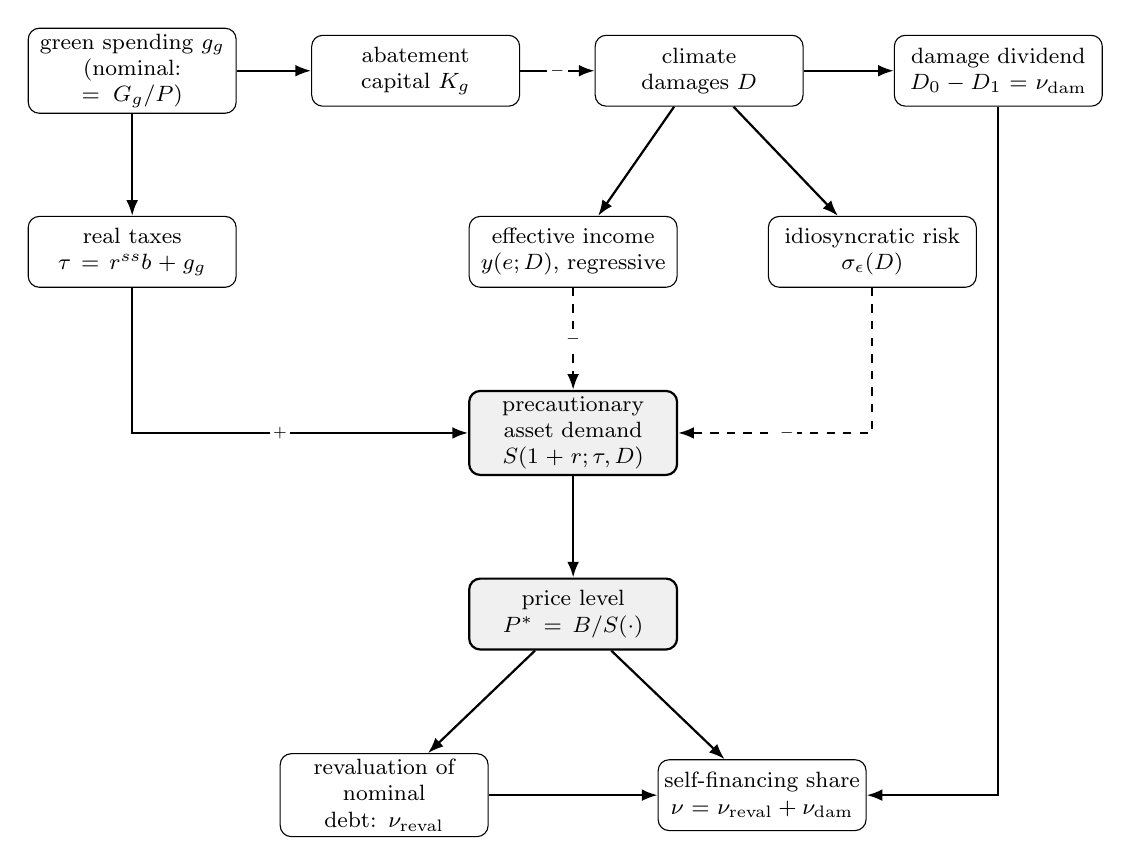
\begin{tikzpicture}[
  font=\footnotesize,
  every node/.style={align=center},
  box/.style={draw, rounded corners, align=center, minimum height=9mm,
              text width=25mm, inner sep=2pt},
  keynode/.style={box, draw=black, thick, fill=black!6},
  arr/.style={-{Latex[length=2mm]}, thick},
  negarr/.style={arr, dashed},
  lbl/.style={font=\tiny, fill=white, inner sep=1pt},
]
 % ---- row 1: climate block (left to right) ----
 \node[box]    (gg)    at (0,0)    {green spending $g_g$\\ \footnotesize(nominal: $=G_g/P$)};
 \node[box]    (kg)    at (3.6,0)  {abatement capital $K_g$};
 \node[box]    (dmg)   at (7.2,0)  {climate damages $D$};
 \node[box]    (nudam) at (11.0,0) {damage dividend\\ $D_0-D_1=\nu_{\mathrm{dam}}$};

 % ---- row 2: climate -> household channels, and real taxes ----
 \node[box] (tau)  at (0,-2.3)   {real taxes\\ $\tau=r^{ss}b+g_g$};
 \node[box] (inc)  at (5.6,-2.3) {effective income\\ $y(e;D)$, regressive};
 \node[box] (risk) at (9.4,-2.3) {idiosyncratic risk\\ $\sigma_\epsilon(D)$};

 % ---- row 3: the market that clears everything above ----
 \node[keynode] (S) at (5.6,-4.6) {precautionary asset demand\\ $\Sfun(1+r;\tau,D)$};

 % ---- row 4: the price level ----
 \node[keynode] (P) at (5.6,-6.9) {price level\\ $P^{*}=B/\Sfun(\cdot)$};

 % ---- row 5: what the price level does ----
 \node[box] (reval) at (3.2,-9.2) {revaluation of\\ nominal debt: $\nu_{\mathrm{reval}}$};
 \node[box] (nu)    at (8.0,-9.2) {self-financing share\\ $\nu=\nu_{\mathrm{reval}}+\nu_{\mathrm{dam}}$};

 % ---- main forward chain (a pure DAG; no feedback drawn -- see text) ----
 \draw[arr] (gg) -- (kg);
 \draw[arr] (kg) -- (dmg) node[lbl, midway] {$-$};
 \draw[arr] (gg) -- (tau);
 \draw[arr] (dmg) -- (inc);
 \draw[arr] (dmg) -- (risk);
 \draw[arr] (dmg) -- (nudam);
 \draw[arr] (S) -- (P);
 \draw[arr] (reval) -- (nu);
 \draw[arr] (P) -- (reval);
 \draw[arr] (P) -- (nu);
 \draw[arr] (nudam.south) |- (nu.east);

 % ---- signed channels into asset demand ----
 \draw[arr]    (tau.south)  |- (S.west)       node[lbl, pos=0.72] {$+$};
 \draw[negarr] (inc.south)  -- (S.north)      node[lbl, midway]   {$-$};
 \draw[negarr] (risk.south) |- (S.east)       node[lbl, pos=0.72] {$-$};
\end{tikzpicture}
\caption{The mechanism. Solid arrows are levels; dashed arrows carry a
sign (marked $-$/$+$) rather than a level. Both climate channels
(effective income, idiosyncratic risk) push precautionary asset demand
\emph{down}; the tax channel pushes it \emph{up}; the price level clears
the difference and revalues the outstanding nominal debt stock
accordingly. Two further channels, discussed in the text but omitted
here for legibility: the \emph{financing instrument} (which tax raises
$\tau$, and from whom) does not touch the climate block above but flips
the sign of $\nu_{\mathrm{reval}}$ (Proposition~\ref{prop:financingdesign});
and, under a nominal budget, the price level \emph{feeds back} into next
period's real spending $g_g=G_g/P$, the loop the transition of
Section~\ref{subsec:tier2} traces out over time.}
\label{fig:mechanism}
\end{figure}

% ==========================================================================
\section{Theoretical results}\label{sec:theory}
% ==========================================================================

Throughout, Assumption~\ref{ass:feasible} holds.

\begin{assumption}\label{ass:feasible}
$\beta(1+r^{ss})<1$, and the feasibility set
$\{P:\ \tau(P) < \min_e y(e;D(P)) + r^{ss}\underline a\}$ is nonempty.
\end{assumption}

% --------------------------------------------------------------------------
\subsection{Preliminaries}

\begin{lemma}[Regularity and scaling of asset demand]\label{lem:S}
On the feasibility set, $\Sfun(1+r;\tau,D)$ is well-defined and continuous in
$(\tau,D)$. With $\phi_D=\psi=0$, CRRA homogeneity gives the exact scaling
\begin{equation}
\Sfun(1+r;\tau,D) = (1-D)\,\Sfun\!\Big(1+r;\ \frac{\tau}{1-D},\ 0\Big):
\label{eq:scaling}
\end{equation}
damages act as a proportional level contraction plus an effective tax
increase. With $\psi>0$ or $\phi_D>0$, $D$ additionally moves the riskiness
of effective income, and $D$ is a genuine second argument.
\end{lemma}

\begin{lemma}[Climate block]\label{lem:climate}
The fixed point \eqref{eq:climatefixedpoint} exists and is unique for every
$g_g\ge0$, and $D(g_g)$ is continuous and strictly decreasing (strictly, when
$\theta_g\alpha_A>0$). Under the nominal budget regime, $P\mapsto D(G_g/P)$
is therefore strictly increasing; under the real mandate it is constant.
\end{lemma}

\begin{lemma}[Nominal anchor]\label{lem:anchor}
In any stationary equilibrium with the nominal growth rule
\eqref{eq:nominalrule}, $\pi^{ss}=\mu$ and $1+r^{ss}=(1+i^{ss})/(1+\mu)$:
policy pins the real rate independently of $P$, so all price-level
determination runs through the single equation $\Phi(P)=0$.
(\citealp{hagedorn2026dtpl}.)
\end{lemma}

% --------------------------------------------------------------------------
\subsection{Determinacy}

\begin{proposition}[Existence and green determinacy]\label{prop:determinacy}
Suppose $\theta_g=0$, or the green budget is indexed. Under
Assumption~\ref{ass:feasible}:
(i) a stationary green equilibrium exists;
(ii) if $\varepsilon_S(P)>-1$ on the feasibility set, it is unique;
(iii) the climate block adds only real, recursively determined objects
$(K_g, X, D)$ and does not alter (i)--(ii).
\end{proposition}

The economic content of (iii) parallels the capital extension in
\citet{hagedorn2026dtpl}: real state variables added to the economy absorb
real equations; the asset market keeps its one job of pricing nominal debt.

% --------------------------------------------------------------------------
\subsection{Self-financing and the sign of the revaluation channel}

\begin{proposition}[Self-financing decomposition]\label{prop:selffinancing}
(i) $\nu=\nu_{\mathrm{reval}}+\nu_{\mathrm{dam}}$ exactly, with
$\nu_{\mathrm{reval}} = r^{ss}B(1/P_0-1/P_1)/g_{g,1}$ and
$\nu_{\mathrm{dam}}=(D_0-D_1)/g_{g,1}$.
(ii) For a marginal program $dG_g>0$ around the no-program steady state, with
$\kappa \equiv -\partial D/\partial g_g \ge 0$ the marginal damage dividend
and $\epsilon_P \equiv d\ln P/dg_g$ the equilibrium price response, the net
burden changes by
\begin{equation}
dN \;=\; \big(1-\kappa\big)\,dg_g \;-\;
\big(\tau^{*}-\kappa\, g_g\big)\,\epsilon_P\, dg_g ,
\label{eq:marginal}
\end{equation}
so the program is marginally self-financing iff
$\kappa + (\tau^{*}-\kappa g_g)\,\epsilon_P \ge 1$; in particular $\kappa\ge1$
suffices regardless of the price response.
(iii) The one-time revaluation $L=B/P_0-B/P_1$ falls on bondholders in
proportion to holdings; because wealth is more concentrated than income in
the invariant distribution, $|L|$ is progressive when positive and regressive
when negative.
\end{proposition}

\begin{result}[Green disinflation]\label{res:disinflation}
$\nu_{\mathrm{reval}}<0$ iff $P_1<P_0$ iff
$\Sfun(1+r^{ss};\tau_1,D_1) > \Sfun(1+r^{ss};\tau_0,D_0)$: the revaluation
channel \emph{subsidizes} bondholders whenever the program raises aggregate
asset demand. Sufficient conditions: $\partial\Sfun/\partial\tau\ge0$
(the constraint-tightening precautionary effect of lump-sum taxes, which the
benchmark calibration exhibits; see Section~\ref{sec:quant}) together with a
damage dividend that does not lower demand. Under the opposite sign
--- $\partial\Sfun/\partial\tau<0$, as in Hagedorn's Result 1 under his
conditions --- a sufficiently tax-heavy program is inflationary and
$\nu_{\mathrm{reval}}>0$, the \citet{angeletos2024deficits} configuration.
The sign of the revaluation channel is thus an \emph{empirically diagnosable}
object, governed by the slope of asset demand in the tax burden.
\end{result}

% --------------------------------------------------------------------------
\subsection{Climate sunspots and anchor insulation}

\begin{proposition}[Climate sunspots]\label{prop:sunspots}
Under the nominal budget regime, suppose the damage--incidence feedback is
strong enough that $\varepsilon_S(P)<-1$ on an open interval intersected by
the demand curve, with the boundary conditions of
Proposition~\ref{prop:determinacy}(i) holding. Then $\Phi$ has at least two
zeros $P_L^{*}<P_H^{*}$: a \emph{green boom} (high real abatement, low
damages and risk) and a \emph{brown stagnation} (low abatement, high damages
and risk). With $\psi>0$ or $\phi_D>0$ the equilibria are Pareto-ranked by
utilitarian welfare, yet each is self-fulfilling: expecting the high price
level means expecting low abatement and high damages concentrated on
constrained households, whose precautionary response validates the high price
level, and conversely. The strategic complementarity is
\begin{equation*}
\text{beliefs about } P \ \longrightarrow\ g_g=\tfrac{G_g}{P}
\ \longrightarrow\ D,\ \sigma_\epsilon(D),\ \chi\text{-incidence}
\ \longrightarrow\ \Sfun \ \longrightarrow\ P=\tfrac{B}{\Sfun}.
\end{equation*}
\end{proposition}

The incidence gradient $\psi$ is quantitatively central here: it determines
whether the damage channel of $\varepsilon_S$ is strong enough to cross $-1$.
With $\psi=0$ the level and risk effects of $D$ on $\Sfun$ largely offset in
the benchmark (Section~\ref{sec:quant}); with $\psi>0$ damages fall on the
households whose buffers respond most, steepening the feedback.

\begin{proposition}[Anchor insulation]\label{prop:insulation}
Under the real mandate, $D$ is constant in $P$ (Lemma~\ref{lem:climate}), so
$\varepsilon_S(P) = \eta_\tau\, d\ln\tau/d\ln P$ with
$d\ln\tau/d\ln P = -\,r^{ss}b/\tau \in(-1,0]$; hence
$|\varepsilon_S|\le|\eta_\tau|$, and if the tax elasticity satisfies
$|\eta_\tau|<1$ --- a magnitude verified numerically at the benchmark --- the
equilibrium is unique for \emph{every} $\theta_g$, $\psi$, $\phi_D$.
\end{proposition}

\begin{corollary}[Greenness of the nominal anchor]\label{cor:anchor}
Determinacy requires insulating the nominal anchor from the climate loop:
keep \emph{debt} nominal (Lemma~\ref{lem:anchor} provides the anchor), and
\emph{index} the green budget (removing the loop).
\end{corollary}

\begin{corollary}[Rule-ranking reversal]\label{cor:reversal}
Without the climate loop, nominal-growth rules guarantee uniqueness for any
shape of $\Sfun$ \citep{hagedorn2026dtpl}; with the loop, the guarantee
survives only for indexed spending. The ranking of nominal versus indexed
rules is reversed for the spending line and unchanged for debt.
\end{corollary}

\begin{corollary}[Missing-anchor corner]\label{cor:sargentwallace}
Full indexation (real debt \emph{and} real spending) removes every nominal
object from \eqref{eq:assetmarket}; $P$ is then indeterminate for the
classical reason \citep{sargentwallace1975}. Insulation concerns \emph{where}
the anchor sits, not whether there is one.
\end{corollary}

% --------------------------------------------------------------------------
\subsection{Optimal accommodation}

\begin{proposition}[Optimal nominal growth]\label{prop:optimalmu}
Let $W(\mu)=\int V\,\dd\Omega$ be utilitarian steady-state welfare along the
nominal growth rate, holding $i^{ss}$ fixed. At the fiscal margin, an increase
in $\mu$ (i) lowers $r^{ss}$ and the real interest burden $r^{ss}b$ --- a
transfer from bondholders, whose wealth-weighted marginal utility is low, to
taxpayers, whose population-weighted marginal utility is high; (ii) raises
$P$, eroding $g_g=G_g/P$ and hence raising $D$ and risk; (iii) lowers the
return on the buffer asset. If bond wealth is more concentrated than income,
the first effect is first-order at small $\mu$ while the climate cost is
proportional to the program size; the optimum $\mu^{*}$ is then interior and
strictly positive. Its magnitude is quantitative.
\end{proposition}

% --------------------------------------------------------------------------
\subsection{Financing design and the revaluation channel}\label{subsec:financingdesign}

\begin{proposition}[Financing design controls the revaluation channel]
\label{prop:financingdesign}
Fix the real program $g_g$ and consider financing mixes
$(\tau_{ls}, \vartheta)$ satisfying the aggregate budget identity
$\tau_{ls} + \vartheta\,(1-D) = r^{ss} b + g_g$, where $\vartheta$ is a
proportional levy on effective endowments. Suppose (i)
$\partial \Sfun/\partial \tau_{ls} \ge 0$ (the constraint-floor
precautionary response to lump-sum taxes, the sign measured at the
benchmark), and (ii) $\Sfun$ inherits the approximate degree-one scaling of
Lemma~\ref{lem:S} in the proportional factor $(1-\vartheta)$. Then a
budget-neutral shift of financing from the lump-sum component toward the
levy lowers aggregate asset demand, raises the equilibrium price level, and
raises $\nu_{\mathrm{reval}}$; augmenting the levy with a lump-sum rebate
(so $\tau_{ls}$ falls below the interest burden) strengthens the shift. In
particular, the sign of the revaluation channel is an instrument of fiscal
design, not a structural constant of green deficits. \emph{[Mechanism proved
under the stated sign conditions; magnitudes quantitative
(Section~\ref{subsec:regimes}).]}
\end{proposition}

% ==========================================================================
\section{Quantitative analysis}\label{sec:quant}
% ==========================================================================

% --------------------------------------------------------------------------
\subsection{Calibration}

The household block inherits the replication benchmark of the underlying DTPL
package: annual frequency, $\beta=0.96$, $\sigma=2$, $\bar a=0$, a 7-state
Rouwenhorst chain with $\rho=0.90$, $\sigma_{\epsilon,0}=0.20$ (unit mean),
$B=1$, $i^{ss}=0.04$, baseline $\mu=0.02$ (so $r^{ss}=0.0196$). The climate
block is \emph{illustrative}: $D_0=0.10$ (no-abatement damages of 10\% of
endowments, within the range that \citealp{bilalkanzig2024} argue is
conservative), $\theta_g=1.2$, $\delta_g=0.10$, risk channel $\phi_D=0.5$,
nominal green budget $G_g=0.012$ (real spending of roughly 5--6\% of mean
endowment at the equilibrium price level). Version-2 climate parameters:
$D_{\max}=0.25$, $\varepsilon_0=1$, $\delta_x=0.05$, $\gamma_x=0.028$,
$\alpha_A=0.9$; incidence $\psi\in\{0,1,2\}$. Numerical method in
Appendix~\ref{app:numerics}.

% --------------------------------------------------------------------------
\subsection{Benchmark results}

Table~\ref{tab:benchmark} reports the benchmark run (authors' full-resolution
run, $n_a=500$; all numbers regenerated by \texttt{main\_project\_run\_all.m}).

\begin{table}[ht]
\centering
\caption{Benchmark quantitative results ($n_a=500$ run).}
\label{tab:benchmark}
\begin{tabular}{lcc}
\toprule
 & no program & green program \\
\midrule
price level $P^{*}$            & 0.2226 & 0.1897 \\
damages $D$                    & 0.1000 & 0.0468 \\
real green spending $g_g$      & 0      & 0.0633 \\
real taxes $\tau$              & 0.0881 & 0.1666 \\
utilitarian welfare $W$        & $-7.807$ & $-8.954$ \\
\midrule
self-financing $\nu$           & \multicolumn{2}{c}{$0.600$} \\
\quad revaluation $\nu_{\mathrm{reval}}$ & \multicolumn{2}{c}{$-0.241$} \\
\quad damage dividend $\nu_{\mathrm{dam}}$ & \multicolumn{2}{c}{$0.841$} \\
one-time revaluation $L$       & \multicolumn{2}{c}{$-0.778$ (bondholder windfall)} \\
\bottomrule
\end{tabular}
\end{table}

Three observations. First, the program is strongly but not fully
self-financing: $\nu=0.60$. Second --- the sign surprise of
Result~\ref{res:disinflation} --- the entire financing contribution comes from
the damage dividend; the revaluation channel is \emph{negative} because the
program is disinflationary ($P$ falls by 15\%): avoided damages raise
effective incomes, and the higher taxes that service the program strengthen
precautionary saving (the measured benchmark has
$\partial\Sfun/\partial\tau>0$; see the interpolant nodes in the run log,
where $\Sfun$ rises from $3.49$ to $5.80$ as $\tau$ moves from $-0.05$ to
$0.22$ at $D=0$). Both forces raise $\Sfun$, and $P=B/\Sfun$ falls.
Bondholders receive a one-time windfall $|L|=0.78$ --- 78\% of annual mean
income --- concentrated at the top of the wealth distribution. Green deficits
in this economy transfer resources \emph{to} rentiers, not from them: the
mirror image of the inflation-erosion intuition, with the opposite
distributional politics. Third, the naive welfare comparison
($W_1<W_0$) is not the policy-relevant object --- it compares steady states
with different tax burdens, ignoring transition gains from lower damages
accruing along the path; the optimal-policy exercise below chooses among
program designs directly.

Figure~\ref{fig:pfig2}(b) traces $\nu(\theta_g)$: the damage dividend is the
engine, and full self-financing $\nu\ge1$ arrives at
$\theta_g\approx2.4$. At $\theta_g=0$ (pure resource cost, no abatement
payoff) $\nu=-0.275<0$: an unproductive nominal program is \emph{worse} than
its sticker price, again because of the disinflationary asset-demand
response.

\pfigguard{PFig1_green_steady_state.pdf}{%
\begin{figure}[ht]\centering

\includegraphics[width=0.6\textwidth]{PFig1_green_steady_state.pdf}
\caption{The green steady state: asset demand and bond supply in
(assets, price-level) space; the dot marks $(B/P^{*},P^{*})$.}
\label{fig:pfig1}
\end{figure}}

\pfigguard{PFig2_self_financing.pdf}{%
\begin{figure}[ht]\centering

\includegraphics[width=0.95\textwidth]{PFig2_self_financing.pdf}
\caption{Self-financing. (a) Decomposition at the benchmark:
$\nu_{\mathrm{reval}}=-0.241$, $\nu_{\mathrm{dam}}=0.841$, $\nu=0.600$.
(b) $\nu(\theta_g)$ crosses full financing near $\theta_g\approx2.4$.}
\label{fig:pfig2}
\end{figure}}

% --------------------------------------------------------------------------
\subsection{Determinacy diagnostics and the sunspot region}

At the benchmark, the equilibrium is unique for every $\theta_g\le2.5$ under
\emph{both} regimes (Figure~\ref{fig:pfig3}): the measured demand elasticity
never crosses $-1$. The diagnostic explains why, and where to look. The tax
channel contributes $\varepsilon_S \approx -\eta_\tau$ with
$\eta_\tau\approx0.3$ at the benchmark; the damage channel is small because,
with $\psi=0$, the \emph{level} effect of damages on demand (negative, by the
scaling in Lemma~\ref{lem:S}) and the \emph{risk} effect (positive, via
$\phi_D$) nearly offset --- visible directly in the interpolant nodes, where
$\Sfun$ is almost flat in $D$ at fixed $\tau$. The sunspot region of
Proposition~\ref{prop:sunspots} therefore requires the \emph{incidence}
gradient: with $\psi>0$, damages compress the incomes of
constraint-adjacent households, whose effective floor drops and whose demand
response is largest --- steepening $d\Sfun/dD$ and pushing
$\varepsilon_S$ toward $-1$ for large programs. The extended experiments
(\texttt{main\_project\_extended.m}) sweep $\psi\in\{0,1,2\}$ and a doubled
program, at the accommodative stance $\mu_{\mathrm{ext}}=0.03$ and with the
carbon-stock climate sector. Table~\ref{tab:frontier} reports the measured
frontier.

\begin{table}[ht]
\centering
\caption{The multiplicity frontier (extended run, $n_a=500$,
$\mu_{\mathrm{ext}}=0.03$, carbon-stock sector). ``0*'' = no stationary
equilibrium exists: $\Phi>0$ at every feasible price level (fiscal-space
collapse), verified by same-sign finite boundaries, not a scan artifact.}
\label{tab:frontier}
\begin{tabular}{ccccc}
\toprule
$\psi$ & $G_g$ & roots (nominal budget) & $\min_P \varepsilon_S$ & roots (mandate) \\
\midrule
0 & 0.012 & 1 & $-0.48$ & 1 \\
0 & 0.024 & 1 & $-0.49$ & 1 \\
1 & 0.012 & 1 & $-0.41$ & 1 \\
1 & 0.024 & 1 & $-0.40$ & 1 \\
2 & 0.012 & 1 & $-0.33$ & 1 \\
2 & 0.024 & 0* & $-0.38$ & 0* \\
\bottomrule
\end{tabular}
\end{table}

Two honest conclusions follow. First, \emph{the sunspot region is empty at
the illustrative benchmark}: the measured demand elasticity never falls
below $-0.49$, far from the $-1$ threshold of
Proposition~\ref{prop:sunspots}. Multiplicity therefore remains a
sufficient-condition result in this paper, not a quantitative claim; whether
empirically disciplined incidence and program scales can reach the threshold
is a calibration question we flag for the next pass. Second --- and more
striking --- what strong incidence produces at this calibration is not two
equilibria but \emph{none}: at $\psi=2$ with the doubled program (and,
in the baseline run, at the tight stance $\mu=0.015$), asset demand exceeds
the real value of debt at every price level for which the tax burden is
feasible. Regressive climate damages do not merely select among equilibria;
they can destroy the fiscal space on which the stationary equilibrium
rests --- a collapse that indexation alone does not repair
(the mandate columns fail at the same point) but accommodation does
(all $\psi\le2$ rows with the benchmark program are unique and interior at
$\mu_{\mathrm{ext}}=0.03$).

\pfigguard{PFig3_sunspots_vs_mandate.pdf}{%
\begin{figure}[ht]\centering

\includegraphics[width=0.95\textwidth]{PFig3_sunspots_vs_mandate.pdf}
\caption{Determinacy diagnostics at $\theta_g=2.5$: (a) $\Phi(P)$ under the
nominal budget and the real mandate; (b) measured $\varepsilon_S(P)$ against
the $-1$ line.}
\label{fig:pfig3}
\end{figure}}

% --------------------------------------------------------------------------
\subsection{The extended sector and accommodation neutrality}

The extended run (carbon-stock climate sector, incidence $\psi=1$,
accommodative stance $\mu_{\mathrm{ext}}=0.03$) delivers a unique interior
green steady state: $P^{*}=0.2826$, $D=0.0709$ (against no-abatement damages
$D(0)=0.0991$), $\tau=0.0768$. Its self-financing decomposition sharpens the
benchmark's message:
\[
\nu = 0.659, \qquad \nu_{\mathrm{reval}} = -0.005, \qquad
\nu_{\mathrm{dam}} = 0.664,
\]
with a one-time bondholder revaluation of only $-0.02$ (against $-0.78$ at
the baseline stance $\mu=0.02$). \emph{Accommodation neutralizes the
revaluation channel}: near the welfare-preferred stance, the no-program and
program price levels nearly coincide ($P_0=0.2842$ vs $P_1=0.2826$), the
program is approximately price-level neutral, and self-financing is almost
entirely the damage dividend. The disinflationary bondholder windfall of the
tight-money benchmark is thus not a fixture of green deficits but a property
of the monetary-fiscal stance --- tight stances hand the revaluation to
bondholders; accommodative stances extinguish it. Under the extended sector
the full self-financing threshold also falls: $\nu(\theta_g)$ crosses one
between $\theta_g=1.5$ ($\nu=0.82$) and $\theta_g=2.0$ ($\nu=1.06$), i.e.\
at $\theta_g\approx1.9$ versus $\approx2.4$ in the reduced-form benchmark,
while an unproductive program remains worse than its sticker price
($\nu=-0.11$ at $\theta_g=0$).

% --------------------------------------------------------------------------
\subsection{Optimal accommodation}

Figure~\ref{fig:pfig4} traces $W(\mu)$. Welfare is hump-shaped with an
interior optimum $\mu^{*}=0.045$ ($W=-7.681$), against a baseline of
$\mu=0.02$ ($W=-8.981$): the optimal policy accommodates the green program
with roughly $4.5\%$ steady-state inflation. The mechanism matches
Proposition~\ref{prop:optimalmu}: moving from $\mu=0.02$ to $0.045$ cuts the
real rate from $2.0\%$ to $-0.5\%$, the real interest burden collapses
($\tau$ falls from $0.167$ to $0.011$ despite unchanged real green spending
financed within the budget), and the price level roughly triples so real
green spending per unit of nominal budget falls --- at $\mu>0.045$ the
climate erosion and the lower buffer return dominate and welfare declines.
At $\mu=0.015$ no equilibrium exists on the scan range: with $r^{ss}$ that
close to the $1/\beta-1$ asymptote, asset demand exceeds $B/P$ at every
feasible price level --- the existence failure the theory predicts, reported
honestly by the solver rather than smoothed over.

\pfigguard{PFig4_optimal_policy.pdf}{%
\begin{figure}[ht]\centering

\includegraphics[width=0.6\textwidth]{PFig4_optimal_policy.pdf}
\caption{Utilitarian welfare $W(\mu)$; the star marks $\mu^{*}=0.045$.}
\label{fig:pfig4}
\end{figure}}

% --------------------------------------------------------------------------
\subsection{The calibrated pass: low, medium, and high damages}
\label{subsec:calibrated}

The results above use the illustrative benchmark, whose fiscal scale is
deliberately large (real debt of roughly five times mean income; a program of
5--6\% of income). The calibrated pass re-targets both margins and
disciplines damages externally: the discount factor is chosen by bisection so
that no-program real debt equals $1.10$ times mean income (OECD
general-government debt/GDP), giving $\beta^{*}=0.9267$; the program is
scaled to real green spending of $2.0\%$ of mean income at the calibrated
price level (the public share of net-zero investment paths); and the
no-abatement damage level takes three externally disciplined values ---
\textbf{low} $D_0=0.02$ (DICE/\citealp{nordhaus2017}), \textbf{medium}
$D_0=0.06$ (the \citealp{golosov2014}-era empirical range of
Dell--Jones--Olken and Burke--Hsiang--Miguel temperature-damage estimates),
and \textbf{high} $D_0=0.20$ \citep{bilalkanzig2024}. Abatement productivity
$\theta_g$ remains illustrative and is reported as a sweep.
Table~\ref{tab:calibrated} reports the run.

\begin{table}[ht]
\centering
\caption{Calibrated self-financing by damage column
($\beta^{*}=0.9267$, debt/income $=1.10$, program $=2\%$ of income,
$\mu=0.02$, $n_a=500$ run, calibration-consistent risk channel). The
$\theta_g$-threshold and welfare rows are from the previous calibration
vintage ($\beta^{*}=0.9296$) and refresh with the next full sweep.}
\label{tab:calibrated}
\begin{tabular}{lccc}
\toprule
 & LOW (DICE) & MEDIUM (DJO--BHM) & HIGH (Bilal--K\"anzig) \\
\midrule
no-abatement damages $D_0$    & 0.02   & 0.06   & 0.20 \\
price level $P_0 \to P_1$     & $0.925 \to 0.876$ & $0.904 \to 0.859$ & $0.855 \to 0.809$ \\
damages $D_0 \to D_1$         & $0.020 \to 0.016$ & $0.060 \to 0.047$ & $0.200 \to 0.153$ \\
real taxes $\tau_1$           & 0.043  & 0.044  & 0.047 \\
\midrule
$\nu$                          & \textbf{0.156} & \textbf{0.583} & \textbf{2.045} \\
\quad revaluation              & $-0.057$ & $-0.053$ & $-0.058$ \\
\quad damage dividend          & $0.212$  & $0.636$  & $2.104$ \\
bondholder windfall $|L|$      & 0.060  & 0.057  & 0.067 \\
full financing at $\theta_g$   & none ($\nu\!=\!0.32$ at $2.5$) & $\approx 2.35$ & $\approx 0.57$ \\
steady-state welfare $W_0 \to W_1$ & $-3.22 \to -3.72$ & $-4.09 \to -4.42$ & $-7.82 \to \mathbf{-7.23}$ \\
\bottomrule
\end{tabular}
\end{table}

Four conclusions. First --- the paper's central conditional statement ---
\emph{whether green deficits finance themselves is a climate-damage
question}: at a defensible fiscal scale, the self-financing share runs from
$0.16$ under conservative DICE damages, through $0.58$ under the empirical
temperature-damage range, to $2.0$ --- full self-financing twice over ---
under high-damage estimates. The model does not claim green deficits are
self-financing; it locates the damage regime in which they are. Second,
under DICE damages \emph{no} abatement productivity in the swept range
delivers full financing ($\nu = 0.32$ even at $\theta_g = 2.5$): the
conservative-damage case is a genuine fiscal cost, which is the honest
counterpart to the high-damage case. Third, \textbf{green disinflation is
robust to the calibration}: the revaluation term is $-0.05$ to $-0.06$ in
every column --- the program lowers the price level by about $5\%$ and hands
bondholders a windfall of $6$--$7\%$ of annual mean income at every damage
level. The sign reversal of the deficit-erosion channel is not an artifact
of the oversized illustrative benchmark. Fourth, in the high-damage column
the program raises steady-state welfare outright ($W$: $-7.82 \to -7.23$)
even before counting transition gains --- avoided damages and reduced
climate risk dominate the added tax burden --- whereas in the low and medium
columns steady-state welfare falls and the case for the program rests on the
transition and on distributional weights, which is precisely where the
welfare-incidence analysis (Section~\ref{subsec:welfaregroups}) and the
dynamic extension take over.

\pfigguard{PFig7_calibrated_nu.pdf}{%
\begin{figure}[ht]\centering

\includegraphics[width=0.6\textwidth]{PFig7_calibrated_nu.pdf}
\caption{Calibrated self-financing by damage column: stacked revaluation
(negative) and damage-dividend components against the full-financing line.}
\label{fig:pfig7}
\end{figure}}

% --------------------------------------------------------------------------
\subsection{Why the price level moves: the safe-asset channel isolated}
\label{subsec:safeasset}

The green disinflation result invites an obvious question: \emph{which}
part of the program moves the price level --- the taxes that pay for it,
the damages it avoids, the income risk it removes, or the instrument that
finances it? The steady-state equilibrium condition $P^{*} = B/S(1+r^{ss})$
makes this answerable by exact counterfactuals: we re-solve the economy
switching on one margin at a time and decompose
$\ln P_1 - \ln P_0$ into a tax-burden contribution (program cost, no
climate benefits), a damage level-and-incidence contribution (damages at
the program level, risk held fixed), a risk contribution (income-risk
level at the program value, endowments held fixed --- the $\phi_D$
channel), and an interaction term reported explicitly rather than absorbed.
Each counterfactual is a well-posed economy whose own budget identity
holds, so no node relies on off-equilibrium objects; the financing
contribution is the levy-versus-lump-sum swap at the same program.
[STEADY STATE; verified run, $n_a = 500$, medium damages, calibrated
scale.]

The verified run decomposes the total green disinflation of
$\ln P_1 - \ln P_0 = -5.72\%$ (from $P_0 = 0.8246$ to $P_1 = 0.7788$)
into:
\[
\underbrace{-7.68\%}_{\text{tax burden}}
\;\underbrace{-\,1.59\%}_{\text{damage level/incid.}}
\;\underbrace{+\,2.31\%}_{\text{risk}}
\;\underbrace{+\,1.24\%}_{\text{interaction}},
\]
with partial-equilibrium asset demand moving from $S(\tau_0, D_0) = 1.213$
to $S(\tau_1, D_0) = 1.305$ (taxes), $S(\tau_0, D_1^{\mathrm{lev}}) =
1.230$ (damage level), and $S(\tau_0, D_1^{\mathrm{risk}}) = 1.186$
(risk). Two lessons, one expected and one not. The expected one: the tax
burden dominates --- lump-sum taxes push constraint-adjacent households
toward precautionary saving, asset demand rises, and the price level
falls, which is the core of green disinflation. The unexpected one: the
\emph{two climate channels have opposite signs}. Avoided damages are
themselves disinflationary ($-1.59\%$): richer households save more in
levels, so the damage dividend \emph{amplifies} the bondholder windfall
rather than offsetting it. Only the risk channel works toward inflation
($+2.31\%$): with less climate-driven income risk, precautionary demand
falls. Green disinflation is therefore not a tax artifact --- it survives
even at zero program cost through the damage-level node --- and its only
countervailing force is the insurance content of climate policy. The
financing swap confirms the regime section at the level of asset demand:
moving the same program from lump-sum to levy financing moves the price
level by $+8.74$ log points, larger than the entire program effect
itself.

\pfigguard{PFig15_safe_asset_decomposition.pdf}{%
\begin{figure}[ht]\centering

\includegraphics[width=0.95\textwidth]{PFig15_safe_asset_decomposition.pdf}
\caption{The safe-asset channel isolated: (a) exact log contributions of
the tax-burden, damage, risk, and interaction margins to
$\ln P_1 - \ln P_0$ (GE counterfactuals); (b) partial-equilibrium asset
demand at the fixed-$(\tau, D)$ nodes.}
\label{fig:pfig15}
\end{figure}}

% --------------------------------------------------------------------------
\subsection{Welfare incidence by wealth group}
\label{subsec:welfaregroups}

Who pays for the program and who benefits? For each state $(a,e)$ we compute
the permanent consumption transfer $\lambda(a,e)$ that makes a household at
that state indifferent between the no-program and program steady states,
aggregated over baseline-distribution wealth quintiles
(Table~\ref{tab:incidence}; generated by \texttt{main\_project\_calibrated}
section C4).

\begin{table}[ht]
\centering
\caption{Consumption-equivalent welfare incidence of the program under
deficit (lump-sum) financing, by baseline wealth quintile (percent;
calibrated pass, $n_a=500$ run).}
\label{tab:incidence}
\begin{tabular}{lccccccc}
\toprule
 & Q1 (poorest) & Q2 & Q3 & Q4 & Q5 & top 10\% & aggregate \\
\midrule
LOW (DICE)          & $-3.57$ & $-2.85$ & $-2.57$ & $-2.28$ & $-1.89$ & $-1.75$ & $-2.64$ \\
MEDIUM (DJO--BHM)   & $-2.60$ & $-1.90$ & $-1.66$ & $-1.42$ & $-1.12$ & $-1.02$ & $-1.75$ \\
HIGH (Bilal--K\"anzig) & $+1.82$ & $+2.33$ & $+2.40$ & $+2.40$ & $+2.29$ & $+2.24$ & $+2.25$ \\
\bottomrule
\end{tabular}
\end{table}

Two findings. First, \textbf{deficit-financed green investment is regressive
at the steady-state margin}: in the low and medium columns the poorest
quintile loses the most ($-3.57\%$ versus $-1.89\%$ for the richest in the
low column), because the lump-sum tax that services the program bites
hardest for households at the borrowing constraint, while the price-level
decline hands the windfall to bondholders at the top. Even in the
high-damage column --- where every quintile gains and the program is a
steady-state Pareto improvement across wealth groups --- the poorest gain
\emph{least} ($+1.82\%$ versus $+2.40\%$ at Q3--Q4), for the same reason. The
distributional politics of green deficits under conventional financing are
therefore inverted relative to the inflation-tax intuition: it is the
\emph{poor} who carry the program and the bondholders who are compensated.
Second, this regressivity is a property of the \emph{financing}, not of the
program --- which motivates the regime comparison below, where the same real
program is financed progressively and the ranking reverses.

\pfigguard{PFig8_welfare_incidence.pdf}{%
\begin{figure}[ht]\centering

\includegraphics[width=0.7\textwidth]{PFig8_welfare_incidence.pdf}
\caption{Welfare incidence by baseline wealth quintile across damage
columns (deficit financing).}
\label{fig:pfig8}
\end{figure}}

\paragraph{Extended groups.} The package additionally reports incidence by
income-state quintile, by bondholding quintile (in the one-asset economy
the only asset \emph{is} the government bond, so wealth and bondholding
quintiles coincide --- a fact worth stating rather than hiding), for
constrained versus unconstrained households, and for a high-MPC proxy
group (the top quartile of the consumption-policy slope $dC/dA$ on the
baseline policy; a proxy, labeled as such). [STEADY STATE; verified run,
medium damages, calibrated scale.] Under \textsc{r1-deficit}, every cut of
the population points the same way: income-state quintiles lose
monotonically ($-3.05\%$, $-2.26\%$, $-1.83\%$, $-1.52\%$, $-1.20\%$ from
bottom to top; exact fractional apportioning of the seven-state process
across quintile boundaries), constrained households ($16.6\%$ of the
population) lose $-2.98\%$ against $-1.77\%$ for the unconstrained, and
the high-MPC quartile loses $-2.54\%$ against $-1.77\%$ for the rest ---
the program under deficit finance is paid for precisely by the households
with the least self-insurance capacity. Under
\textsc{r3-prop-levy-rebate} every one of those orderings \emph{reverses}:
the income quintiles gain $+2.01\%$, $+1.11\%$, $+0.58\%$, $+0.18\%$,
$-0.25\%$ from bottom to top, the constrained gain $+1.89\%$ against
$+0.50\%$, and the high-MPC group $+1.35\%$ against $+0.51\%$, at an
aggregate gain of $+0.73\%$ against the deficit regime's $-1.97\%$.
Stated conditionally: incidence is regressive under pure deficit finance
in the low and medium damage calibrations, rebate financing reverses
bottom-half losses, and in the high-damage column all groups gain --- but
full self-financing remains conditional on the high-damage,
high-effectiveness region.

\pfigguard{PFig16_extended_welfare_groups.pdf}{%
\begin{figure}[ht]\centering

\includegraphics[width=0.95\textwidth]{PFig16_extended_welfare_groups.pdf}
\caption{Extended welfare groups (deficit vs.\ levy-plus-rebate financing):
income-state and wealth(=bondholding) quintiles; constrained and high-MPC
households.}
\label{fig:pfig16}
\end{figure}}

% --------------------------------------------------------------------------
\subsection{Financing regimes: deficit, proportional levy, rebate, mixed}
\label{subsec:regimes}

Green spending is not carbon policy, and financing design is a choice. The
package compares four ways of financing the \emph{same} real program at the
calibrated medium-damage column: (\textsc{r1-deficit}) lump-sum/deficit
financing (the baseline); (\textsc{r2-prop-levy}) a proportional levy on
effective endowments that funds the program; (\textsc{r3-prop-levy-rebate})
the levy at twice the program with half rebated lump-sum (the progressive
rebate design suggested by the incidence evidence in
\citealp{kanzig2023carbon}); and (\textsc{r4-mixed-deficit-levy}) an even
deficit/levy mix. All four satisfy the same aggregate budget identity
$\tau_{ls} + \vartheta\,(1-D) = r^{ss} b + g_g$, so aggregate resources are
identical: the regimes differ only in \emph{incidence} --- proportional
versus lump-sum --- transmitted through precautionary asset demand to the
price level, the self-financing share, and group welfare. In the endowment
HA-DTPL block, the levy should be interpreted as a \emph{proportional
financing instrument with carbon-tax-style incidence}. The Pigouvian
carbon-tax margin requires the clean/dirty production extension and is not
claimed in this section: neither instrument distorts a margin here and the
levy carries no abatement incentive (abatement is public). What this
comparison isolates is the pure incidence-and-price-level content of
financing design --- which, given that the revaluation channel is an
incidence object, is exactly where the DTPL mechanism has bite.
Table~\ref{tab:regimes} reports the run (medium damages, calibrated scale;
no-program baseline $P_0 = 0.8246$).

\begin{table}[ht]
\centering
\caption{Financing regimes for the same real green program
(medium damages, calibrated scale, $n_a=500$ run). $\lambda_{b50}$,
$\lambda_{t10}$: consumption-equivalent gains of the bottom 50\% and top
10\% of the baseline wealth distribution.}
\label{tab:regimes}
\begin{tabular}{lcccccc}
\toprule
Regime & $P^{*}$ & $\nu$ & $\nu_{\mathrm{reval}}$ & $\nu_{\mathrm{dam}}$ &
$\lambda_{b50}$ & $\lambda_{t10}$ \\
\midrule
\textsc{r1-deficit} (lump-sum)      & 0.779 & 0.568 & $-0.060$ & 0.628 & $-2.42\%$ & $-1.15\%$ \\
\textsc{r2-prop-levy}               & 0.850 & 0.668 & $+0.033$ & 0.635 & $-0.41\%$ & $-0.58\%$ \\
\textsc{r3-prop-levy-rebate}        & 0.916 & \textbf{0.759} & $\mathbf{+0.119}$ & 0.641 & $\mathbf{+1.23\%}$ & $-0.13\%$ \\
\textsc{r4-mixed-deficit-levy}      & 0.816 & 0.620 & $-0.012$ & 0.632 & $-1.35\%$ & $-0.84\%$ \\
\bottomrule
\end{tabular}
\end{table}

Three results, the first of which we regard as the sharpest in the paper.
First, \textbf{the sign of the revaluation channel is a policy choice}
(Proposition~\ref{prop:financingdesign}): moving from lump-sum to
proportional financing flips green disinflation ($\nu_{\mathrm{reval}} =
-0.060$) into mild green inflation ($+0.033$; $+0.119$ with the rebate).
The mechanism is the asset-demand incidence at the heart of the DTPL:
lump-sum taxes push constraint-adjacent households toward their borrowing
limit and \emph{raise} precautionary demand (the price level falls, the
fisc loses the revaluation); a proportional levy scales endowments and
\emph{lowers} demand roughly proportionally (the price level rises, real
debt erodes). Second, the progressive design wins on \emph{both} margins
simultaneously: the levy-plus-rebate regime is the most self-financing
($\nu = 0.759$, a fifth more than deficit financing) \emph{and} the most
progressive (the bottom half gains $+1.23\%$ against $-2.42\%$ under
deficit financing, while the top decile is nearly unharmed at $-0.13\%$
versus $-1.15\%$) --- a near-Pareto dominance over the conventional deficit
regime. Third, the magnitudes quantify how much the DTPL incidence channel
is worth: all four regimes purchase the identical real program with
identical aggregate resources, yet the bottom half's welfare differs by
$3.7$ percentage points of permanent consumption between the worst and best
design. Financing structure is not fiscal bookkeeping in this economy; it
is a price-level and distribution instrument.

\pfigguard{PFig9_financing_regimes.pdf}{%
\begin{figure}[ht]\centering

\includegraphics[width=0.95\textwidth]{PFig9_financing_regimes.pdf}
\caption{Financing regimes: (a) self-financing decomposition; (b) welfare
incidence, bottom 50\% versus top 10\%.}
\label{fig:pfig9}
\end{figure}}

% --------------------------------------------------------------------------
\subsection{Bounding the revaluation channel: maturity, indexation, holders}
\label{subsec:maturity}

The inflating-away literature disciplines how much fiscal room nominal-debt
revaluation can really provide: \citet{hilscher2022} show that maturity,
holder composition and the persistence of inflation sharply limit it;
\citet{hallsargent2011} supply the maturity-adjusted accounting;
\citet{doepkeschneider2006} and \citet{auclert2019} the redistribution
mapping. Our framework adds a clarifying twist. In steady-state comparisons
at unchanged $(i,\mu)$, the program moves the price level once --- a
\emph{level jump} --- and a level jump revalues all nominal promises
proportionally \emph{regardless of maturity}: duration neither shields nor
amplifies it. The binding limits are instead (i) \emph{indexation leakage}
--- a share $\alpha_I$ of indexed debt does not revalue, so the fiscal
component scales by $(1-\alpha_I)$; and (ii) \emph{holder composition} ---
a share $\alpha_F$ of foreign-held nominal debt leaves the fiscal gain
unchanged but reallocates the domestic incidence by
$(1-\alpha_I)(1-\alpha_F)$. Because our calibrated revaluation channel is
\emph{negative} (green disinflation), these leakages work in the
government's favor: indexed debt shrinks the fiscal loss, and foreign
holders absorb part of the bondholder windfall that would otherwise accrue
to wealthy domestic households. Duration proper enters only where the real
rate moves --- the accommodation experiments --- through the repricing of
legacy long bonds (geometric-coupon price $q = 1/(1+r-\delta_m)$). The
module \texttt{debt\_maturity\_revaluation.m} reports the maturity-adjusted
share $\nu^{M} = (1-\alpha_I)\,\nu_{\mathrm{reval}} + \nu_{\mathrm{dam}}$
over $\alpha_I \in \{0, 0.10, 0.25\}$, the domestic-incidence table over
$\alpha_F \in \{0, 0.30, 0.50\}$, and the duration term for the
$\mu = 0.02 \to 0.045$ accommodation move at durations of one, five and ten
years; the implementation-efficiency sweep $q_g \in \{0.6, 0.8, 1.0\}$
(planning delays and procurement frictions in the spirit of
\citealp{leeperwalkeryang2010}, disciplined by \citealp{bomligthart2014}
and the IMF's climate public-investment framework) scales the damage
dividend correspondingly.

The run (calibrated medium column) delivers three quantitative statements.
First, because the revaluation channel is negative, \emph{indexation raises
the self-financing share}: $\nu^{M} = 0.563$, $0.570$ and $0.579$ at indexed
shares $\alpha_I = 0$, $0.10$ and $0.25$ --- indexed debt shields the fisc
from the disinflation loss, the mirror image of the usual
inflating-away logic. Second, foreign holders absorb the windfall: the
domestic revaluation incidence shrinks from $-0.058$ to $-0.029$ as the
foreign-held share rises from zero to one half (at $\alpha_I = 0.10$).
Third, duration amplifies who gains from \emph{accommodation}: under the
$\mu = 0.02 \to 0.045$ move the legacy bond repricing alone hands holders
$+2.4\%$ at one-year duration, $+12.5\%$ at five years and $+25.6\%$ at ten
years (holding revaluations including the level effect: $+9.0\%$,
$+19.6\%$, $+33.6\%$) --- accommodation redistributes toward long-bond
holders, in line with the \citet{hallsargent2011} accounting.
Implementation frictions scale the damage dividend nearly linearly:
$\nu = 0.563$, $0.449$ and $0.329$ at $q_g = 1.0$, $0.8$ and $0.6$
(the revaluation component barely moves, $-0.064$ to $-0.069$), so a forty
percent efficiency loss forfeits roughly forty percent of self-financing
--- quantifying why climate public-investment management
(Climate-PIMA-style) is a fiscal issue, not only an engineering one.

\pfigguard{PFig10_maturity_bounds.pdf}{%
\begin{figure}[ht]\centering

\includegraphics[width=0.95\textwidth]{PFig10_maturity_bounds.pdf}
\caption{Bounding the revaluation channel: (a) fiscal $\nu^M$ under
indexation; (b) domestic incidence under foreign holdings.}
\label{fig:pfig10}
\end{figure}}

\pfigguard{PFig11_implementation_qg.pdf}{%
\begin{figure}[ht]\centering

\includegraphics[width=0.6\textwidth]{PFig11_implementation_qg.pdf}
\caption{Implementation efficiency $q_g$ and the damage dividend
(medium damages, calibrated scale).}
\label{fig:pfig11}
\end{figure}}

% ==========================================================================
\section{Transition diagnostics}\label{sec:transitions}
% ==========================================================================

All quantitative results so far are \emph{steady-state} comparisons. This
section reports three tiers of dynamics, each labeled by what it is and
--- more importantly --- by what it is not. The first two are
\textbf{RANK/NK transition diagnostics and tier-1 linearized HANK impulse
responses; they do not implement the nonlinear DTPL price-level
mechanism}: in both blocks inflation dynamics come from a Phillips curve
and a policy rule, not from asset-market clearing of the nominal debt
stock. We report them because they answer two questions the steady-state
analysis cannot: does the announced program destabilize the nominal block
on the way to the new steady state, and how does the answer depend on the
monetary regime? The third tier (Section~\ref{subsec:tier2}) is the
paper's own mechanism in dynamics --- the nonlinear heterogeneous-agent
transition in which the price-level \emph{path} is the unknown pinned by
asset demand, with no Phillips curve anywhere --- and its converged
solution turns the steady-state revaluation result into an announcement
effect: the green disinflation is front-loaded into the announcement
year, and the tier's inflation response has the \emph{opposite sign} to
the linearized tiers', which is precisely the observable content of the
mechanism.

\subsection{RANK/NK transitions under four monetary regimes}
\label{subsec:ranktrans}

[RANK/NK TRANSITION DIAGNOSTIC; IMPLEMENTED, run verified.] A
representative-agent New Keynesian economy with Rotemberg pricing carries
the same climate block as the quantitative model (green public capital
$K_g$, carbon stock $X$, TFP damages $D$; identical parameters). A
permanent green-investment program of the calibrated steady-state scale
phases in linearly over twelve quarters (implementation delays in the
spirit of \citet{leeperwalkeryang2010}) and is financed \emph{contemporaneously by
taxes} under a debt-stabilizing fiscal rule --- by design, so that the
exercise isolates the real/nominal transition shape from the deficit
question studied everywhere else in the paper. Perfect-foresight paths
(300 quarters) are computed under four regimes: a weakly active rule
(\textsc{weak}: $\phi_\pi=1.1$, $\rho_i=0.5$, the closest numerically
regular stand-in for a peg), an inertial Taylor rule (\textsc{taylor}:
$\phi_\pi=1.5$, $\rho_i=0.8$), strict inflation targeting
(\textsc{aggressive}: $\phi_\pi=3$), and a temporary green accommodation
(\textsc{greenaccom}: Taylor plus a rate cut proportional to the
green-capital gap, $\psi_g=0.03$, fading as $K_g$ accumulates). The
accommodation is deliberately large: the un-smoothed stance target implies
a cut of about seven annualized percentage points at the program's start,
though the rule's own inertia ($\rho_i=0.8$) means the realized first-period
cut is nearer one and a half points, building thereafter.

Three findings, all verified by the converged runs (solver residuals
$\sim 10^{-14}$; the $K_g$ accumulation identity holds to $10^{-9}$ on
every reported path):

\begin{enumerate}
\item \emph{The tax-financed program is essentially price-stable under any
active rule.} Impact inflation is $-0.04$\% (annualized) under
\textsc{weak}, $-0.52$\% under \textsc{taylor}, $-0.24$\% under
\textsc{aggressive}; peak inflation along the entire transition stays
below $+1.6$\% annualized in all three. A ramped green program of
realistic scale is not, by itself, an inflationary event in the NK block.
\item \emph{The real green transition is monetary-regime independent.}
Green capital reaches $0.349$ (58\% of its terminal level) after 40
quarters and damages fall from $0.0972$ to $0.0925$ in all three active
regimes --- identical to three decimals. The monetary regime redistributes
the nominal path, not the green capital path.
\item \emph{Accommodation buys inflation, not green capital.} The large
\textsc{greenaccom} experiment produces a $+22.6$\% annualized
impact-inflation spike, yet after 40 quarters green capital is the same
($0.349$) and damages are slightly \emph{higher} ($0.0933$): the
demand boom raises output and hence emissions along the way. In the NK
block, tying rate cuts to the green-capital gap is a pure nominal
intervention --- a transition-dynamics counterpart of the steady-state
accommodation-neutrality result of Section~\ref{sec:quant}, and further
motivation for the anchor-insulation design of
Proposition~\ref{prop:insulation}.
\end{enumerate}

\pfigguard{PFig13_rank_transitions.pdf}{%
\begin{figure}[ht]\centering

\includegraphics[width=0.95\textwidth]{PFig13_rank_transitions.pdf}
\caption{RANK/NK transition diagnostics: perfect-foresight paths for a
permanent tax-financed green program (12-quarter ramp-in) under four
monetary regimes. Scope: these paths do not implement the DTPL
price-level mechanism.}
\label{fig:pfig13}
\end{figure}}

\subsection{Tier-1 HANK impulse responses}\label{subsec:hanktier1}

[TIER-1 LINEARIZED HANK IRF; IMPLEMENTED, run completed on the user
machine; figure below.] The second tier restores household heterogeneity:
a one-asset HANK (borrowing constraint, idiosyncratic efficiency risk)
solved with sequence-space Jacobians in Dynare's heterogeneity framework,
carrying the same climate block, a \emph{nominal} policy rate together
with the ex-post Fisher equation --- so that surprise inflation revalues
household asset positions state by state, the linearized counterpart of
the paper's redistribution channel --- and a slow debt-stabilizing tax
rule, so that a quasi-permanent green-investment expansion (persistence
$0.995$, one percent of steady-state output) is \emph{deficit-financed on
impact}. Discount factor and labor disutility are calibrated to clear the
asset and labor markets at a damaged steady state with debt at the
calibration target of Section~\ref{sec:quant}; the income process is the
three-state benchmark of the framework's reference implementation rather
than the seven-state process of the quantitative model, so magnitudes
here are indicative, not calibrated results.

Its role is deliberately limited: it is the bridge between the RANK
diagnostics and the full nonlinear HANK-DTPL transition, showing that the
qualitative transition shapes survive heterogeneity and Fisher
redistribution. It does not --- and in a linearized NK setting cannot ---
deliver price-\emph{level} determination by asset demand.
Figure~\ref{fig:pfig14} reports the responses of output, inflation, real
debt, green capital, damages, and the ex-post real return under four
monetary regimes analogous to the RANK block's, though not identical to
them: the HANK rules omit interest-rate inertia and the HANK accommodation
keys off the program flow rather than the green-capital gap, so the
\textsc{greenaccom} experiment here is far milder than its RANK namesake
and the two tiers are compared on shapes, not on levels.

The verified run (five regimes solved; calibrated $\beta = 0.9796$;
one-percent-of-output program; persistence $\rho_g = 0.98$) delivers the
tier's key message in two comparisons. \emph{Across monetary rules},
impact inflation is $+2.53\%$ annualized under \textsc{weak}, $+0.44\%$
under \textsc{taylor}, $+0.10\%$ under \textsc{aggressive}, $+0.65\%$
under \textsc{greenaccom}, with output up half a percent of its
steady-state level on impact ($+0.0044$ in levels against $\bar Y =
0.90$) --- positive throughout, against impact deflation in the
tax-financed, ramped RANK experiment of Section~\ref{subsec:ranktrans}
--- and the real green path is again rule-independent (green capital
$+0.148$, damages $-0.0032$ after 40 quarters, identical to three
decimals across all regimes). \emph{Within the Taylor rule}, a fifth
regime (\textsc{taylorbal}) re-runs the identical program with a fast
debt-stabilizing tax rule in place of the slow one, isolating the
deficit-financing component while holding the model fixed: real debt
after 40 quarters rises $+0.007$ instead of $+0.071$ --- the debt buildup
is almost entirely a financing choice --- yet impact inflation barely
moves ($+0.36\%$ against $+0.44\%$). The
decomposition is sharp: in the linearized HANK, \emph{deficit financing
buys the debt path, not the inflation path} --- the mild impact inflation
belongs to the unanticipated program itself, its size is set by the
monetary rule, and the financing margin prices into the fisc's balance
sheet rather than into goods prices. (The steady-state DTPL analysis is
where the financing margin does move the price level --- through
asset-demand incidence, Section~\ref{subsec:safeasset} --- which is
precisely the mechanism a linearized NK Phillips curve cannot represent;
the contrast between the two tiers is thus itself informative.) These
magnitudes are indicative, not calibrated results: the income process is
the framework's three-state benchmark. [TIER-1 LINEARIZED HANK IRF;
validation table \texttt{hank\_tier1\_validation.txt}.]

\pfigguard{PFig14_hank_green_irfs.pdf}{%
\begin{figure}[ht]\centering

\includegraphics[width=0.95\textwidth]{PFig14_hank_green_irfs.pdf}
\caption{Tier-1 HANK: linearized sequence-space impulse responses to a
quasi-permanent deficit-financed green-investment shock (one percent of
steady-state output, persistence $0.98$) under four monetary regimes.
The ex-post real return panel is the linearized Fisher revaluation
channel. Scope: linearized IRFs, not the nonlinear DTPL price-level
transition.}
\label{fig:pfig14}
\end{figure}}

\paragraph{A two-asset tier and its accuracy protocol.} The replication
package also implements a two-asset extension of the HANK tier
(liquid nominal bonds versus illiquid equity with convex
portfolio-adjustment costs, sticky wages and prices, investment with
Tobin's $Q$, and endogenous government debt, so that households'
demand for the liquid nominal asset --- the $B/P$ margin at the heart of
the model --- is observable separately from total wealth). One design
lesson from this tier is itself worth recording: we attempted to make
the liquidity premium an \emph{endogenous convenience yield} clearing
the liquid-bond market, under both natural timings of the premium, and
both are boundary-singular in a truncated sequence-space system --- the
contemporaneous premium has only an income effect on predetermined
holdings at the impact date, while the issuance-timed premium leaves the
terminal-date premium outside every within-horizon equation --- so the
tier closes, like the reference implementation, with a single
total-wealth clearing condition and a constant premium, and the
endogenous convenience yield remains future work. We also flag a
numerical finding rather than hide it: the first solution of this tier
produced visibly \emph{oscillatory} impulse responses. The likely causes are generic to
sequence-space methods --- shock persistence ($0.995$) too close to the
truncation horizon (300 quarters), which produces reflection artifacts,
compounded by the coarse benchmark asset grids of the reference
implementation --- and the package now enforces an explicit accuracy
protocol: an oscillation diagnostic (sign changes of the differenced
response beyond the impact phase), reduced shock persistence with a
longer horizon, and a full refinement re-solve (double grid densities,
horizon 600) that must agree with the baseline to within ten percent
before any number from this tier can be reported. The protocol earned
its keep immediately: the fast-financing regime of the first run
returned an \emph{explosive} pseudo-solution (impact inflation orders of
magnitude too large), which a naive reading would have reported as a
regime result. An adversarial equation-by-equation audit traced it to a
genuine specification error: in adapting the reference two-asset model we
had inherited its steady-state-calibration variant, which omits the firm
cash-flow identity $\mathrm{div}=Y-wN-I-\psi^p$ because it uses both
asset-market clearing conditions as calibration targets. Without that
identity, dividends are defined only residually by the equity-pricing
equation, which collapses the equity return to the safe return
identically and leaves the equity price unanchored while violating
goods-market feasibility out of steady state. The corrected model
restores the identity and closes, as described above, with the single
total-wealth clearing condition and a constant premium. The driver
additionally rejects any path violating elementary plausibility bounds.
The accuracy protocol was then run on the corrected model repeatedly,
and the failure eventually stabilized into a reproducible signature: in
every regime the steady-state calibration converges, and the
sequence-space Jacobian assembly then returns a matrix containing
\texttt{NaN} entries, so no impulse response is ever computed. That
reproducibility made the defect diagnosable, and an equation-level audit
located a concrete mechanism in the reference template itself: the
portfolio-adjustment cost is written with $\mathrm{sign}(\cdot)$ and
$|\cdot|^{\chi_2-1}$ where $\chi_2$ enters \emph{symbolically}, so the
emitted second-derivative code contains factors
$(\chi_2-1)(\chi_2-2)\,|D|^{\chi_2-3}$ with $D$ the deviation from the
no-adjustment portfolio. Households at the illiquid constraint --- a
positive-mass corner by construction --- have $D=0$ exactly, where
$|D|^{\chi_2-3} = 0^{-1} = \infty$ and the $(\chi_2-2)=0$ factor turns
the product into $0\times\infty = \mathrm{NaN}$, precisely inside the
Jacobian evaluation that fails. Because $\chi_2=2$ in the calibration,
every kinked expression equals a smooth polynomial \emph{identically}
($\mathrm{sign}(D)|D|^{\chi_2-1} \equiv D$, $|D|^{\chi_2} \equiv D^2$),
and the model file now carries those exact equivalents (plus the removal
of the template's one exogenous-lead auxiliary). The repaired model
awaits its re-run; until the protocol passes, the tier's driver stops by
default with the recorded verdict. No two-asset result appears in this
paper; the tier is disclosed because a solved-but-wrong impulse response
is worse than an honest gap, and its economics are covered by the
one-asset tier (Fisher redistribution) and the nonlinear tier-2
transition (the $B/P$ margin proper). [TIER-1b: IMPLEMENTED; protocol
failure diagnosed to a reproducible kink-derivative \texttt{NaN} at the
constraint corner; exact smooth repair in place, re-run pending; NOT
REPORTABLE.]

% --------------------------------------------------------------------------
\subsection{The nonlinear HANK-DTPL transition}\label{subsec:tier2}

[NONLINEAR HANK-DTPL TRANSITION; IMPLEMENTED, run VERIFIED: converged and
horizon-adequate at $n_a=500$, $T=80$; all numbers below are from that
residual-verified run.] The tiers above borrow their inflation dynamics
from a Phillips curve. The paper's own mechanism makes a starker
prediction about the transition, and the package computes it. At $t=1$ the government unexpectedly announces
the permanent program; thereafter foresight is perfect. The unknown is
the \emph{price-level path} $\{P_t\}_{t=1}^{T}$: at every date the price
level must clear the asset market,
\[
S_t\bigl(\{r_s, \tau_s, D_s\}_{s \ge t};\, V_T,\, \Omega_t\bigr)
\;=\; \frac{B_t}{P_t}, \qquad
1 + r_t = (1+i^{ss})\,\frac{P_{t-1}}{P_t},
\]
where $S_t$ is exact aggregate asset demand from the household problem
solved \emph{backward} from the green terminal steady state under the
time-varying taxes, damages, and realized real returns implied by the
trial price path, and the wealth distribution $\Omega_t$ rolls
\emph{forward} from the pre-announcement stationary distribution. There
is no Phillips curve and no policy rule for inflation anywhere in this
computation: the inflation path \emph{is} the repricing of the nominal
debt stock against precautionary asset demand, period by period, and the
$t=1$ jump of $P_1$ against the pre-announcement price level is the
surprise revaluation of outstanding nominal positions --- the paper's
channel realized along a path rather than compared across steady states.
Stationarizing by the nominal-growth trend $(1+\mu)^t$ makes the system
autonomous; the terminal condition pins $\hat{P}_T$ at the green
steady-state price level, and the government budget holds by construction
at every trial path ($\tau_t = \bar r\, b_t + g_t$). The solver is an
Anderson-accelerated fixed point on the log price path: the underlying map
moves each $\hat P_t$ toward $B_t/S_t$ (excess asset demand at $t$
\emph{lowers} $\hat P_t$, raising the real value $B_t/P_t$ of the fixed
nominal stock until it meets demand --- the transition form of
$P^{*}=B/S$), and because a change in $\hat P_t$ moves the realized real
return at dates $t$ and $t+1$ with opposite signs --- a cross-date
coupling under which plain diagonal relaxation stalls --- the update
combines the most recent residuals by least squares (type-II Anderson,
memory five), with a per-iteration trust region and the market-clearing
residuals reported at every date. Convergence is assessed on the
\emph{free} unknowns $\hat P_1,\dots,\hat P_{T-1}$; the pinned terminal
date's residual is reported separately as a horizon-adequacy check --- it
vanishes only when $T$ is long enough for the wealth distribution to
reach the green steady state, at which point green-steady-state savings
equal $B_T/P_T$ by construction. A path that is not both converged and
horizon-adequate is returned as such and cannot be presented as a result.
Each iteration costs $T$ exact Bellman steps plus $T$
distribution pushes on the full $(a,e)$ grids --- deliberately the
computationally heaviest object in the package. Two experiments run by
default: the \emph{nominal appropriation} (the anchor-exposed design) and
the \emph{indexed mandate} (the anchor-insulated design of
Proposition~\ref{prop:insulation}); the comparison of their announcement
jumps is the dynamic version of the anchor-insulation result, and the
model's central untested prediction --- that a credible green
announcement produces \emph{disinflation on impact} under deficit
finance --- becomes a computed, sign-testable object
(Section~\ref{sec:empirics}, E3).

The converged run ($n_a = 500$, $T = 80$ years, medium damages, $\beta$
calibrated on this same grid so that pre-announcement real debt matches
the $1.10$ target; interior market-clearing residual below $5\times10^{-4}$
at every free date, terminal residual below $5\times10^{-4}$, $88$ and
$72$ Anderson iterations for the two designs) delivers the paper's
dynamics in three statements. \emph{First, green disinflation is
front-loaded:} the announcement moves the stationarized price level down
$3.9\%$ on impact --- year-one inflation of $-2.0\%$ against the $+2\%$
nominal trend --- which is $77\%$ of the entire long-run green
disinflation ($-5.1\%$ across steady states) realized in the announcement
year, before the first unit of green capital is installed. The price
level jumps because asset demand does: households capitalize the future
damage reduction and the transition-long tax path immediately, and the
price level is what clears that market. Inflation is back within a
quarter-point of trend by year two --- and stays there --- while green
capital accumulates over decades: the announcement effect and the
accumulation dynamics separate cleanly.
\emph{Second, the revaluation channel is a one-time announcement windfall:}
the surprise repricing hands holders of the outstanding nominal stock a
real gain of $5.3\%$ of the program's present value ($5.3\%$ under the
indexed mandate) --- the dynamic realization of the negative
$\nu_{\text{reval}}$ of the steady-state decomposition, collected entirely
in the announcement year. \emph{Third, the denomination of the green
budget is irrelevant on the equilibrium path:} the nominal-appropriation
and indexed-mandate designs produce announcement jumps within two
hundredths of a percentage point of each other and land on the same
terminal steady state, so the anchor-insulation value of the indexed
mandate (Proposition~\ref{prop:insulation}) is entirely
\emph{off}-equilibrium --- it removes the self-fulfilling brown-stagnation
equilibria without changing the equilibrium the economy actually follows.
The contrast with the Phillips-curve tiers is the point of the exercise:
the linearized HANK tier prices a comparable deficit-financed green
announcement (a quasi-permanent program of one percent of output) at
$+0.4\%$ impact inflation (the demand stimulus), while the DTPL
computation prices its permanent program at $-2.0\%$ (the asset-demand
shift) --- opposite signs for the same class of announcement, because the
two tiers answer with different mechanisms, and only the latter contains
the price-level-as-market-clearing margin the paper is about. [NONLINEAR
HANK-DTPL TRANSITION; converged, horizon-adequate, grid-consistent run;
\texttt{transition\_dtpl\_summary.txt}.]

\pfigguard{PFig18_dtpl_transition.pdf}{%
\begin{figure}[ht]\centering

\includegraphics[width=0.95\textwidth]{PFig18_dtpl_transition.pdf}
\caption{The nonlinear HANK-DTPL transition (converged, grid-consistent
run, $n_a=500$, $T=80$ years, $\beta$ calibrated on this grid to the
$1.10$ debt target): stationarized price level, inflation, real debt
versus asset demand, green capital, damages, and market-clearing
residuals, for the nominal-appropriation and indexed-mandate designs. The
announcement jump (the $-3.9\%$ price-level drop between the
pre-announcement level and year one) front-loads $77\%$ of the long-run
green disinflation; inflation is within a quarter-point of the $2\%$
trend by year two; the two designs are nearly indistinguishable on the
equilibrium path. Residuals clear to $5\times10^{-4}$ at every date.
Generated by \texttt{main\_project\_transition}.}
\label{fig:pfig18}
\end{figure}}

% ==========================================================================
\section{Empirical evidence}\label{sec:empirics}
% ==========================================================================

The empirical strategy follows from what the theory does and does not
pin down, and we state its logic before its results. The model makes
three kinds of claims with three different evidentiary standards. First,
an \emph{anchor} claim (Lemma~\ref{lem:anchor}): long-run inflation
equals the growth of nominal fiscal aggregates relative to real output,
slope one, no free parameter --- directly testable in cross-country
panels, and tested below (E1, E4). Second, a \emph{sign} claim unique to
this mechanism: under deficit finance a credible green investment
announcement is \emph{disinflationary} (it raises safe-asset demand),
whereas every sticky-price transition model of the green transition we
are aware of predicts inflation or neutrality --- so announcement-window
breakeven-inflation responses around major green fiscal events can
discriminate between the two mechanism classes (E3), and the nonlinear
transition of Section~\ref{subsec:tier2} turns that sign into a computed
path. Third, a \emph{design} claim: nominal appropriations and indexed
mandates behave differently for determinacy
(Proposition~\ref{prop:insulation}), which motivates a purpose-built
registry of green budget denominations (E2) --- to our knowledge not
assembled anywhere --- rather than an off-the-shelf dataset. We claim
causal identification for none of these; the empirical layer validates
signs, magnitudes, and institutional premises, and we label each result
accordingly.

The model's empirical content comes in three layers.

\paragraph{E1: the nominal anchor (testable now).} Lemma~\ref{lem:anchor}
implies that long-run average inflation equals the long-run growth rate of
nominal fiscal aggregates relative to real output --- slope one, no free
parameter. In the 34-country OECD panel distributed with the replication
package (average CPI inflation against average growth of nominal government
expenditure over real GDP), OLS delivers
\[
\widehat{\pi}_c = \alpha + \beta\, g^{G}_c + u_c, \qquad
\widehat\beta = 1.004 \ \ (\text{HC1 s.e. } 0.257), \qquad n = 34,
\]
with correlation $0.56$ and $R^2 = 0.32$
(\texttt{empirical\_anchor.m}; Figure PFig5). The Wald test of the theory's
sharp prediction $\beta=1$ gives $t = 0.01$, $p = 0.99$: the anchor slope is
almost exactly one and the theory is not rejected. The honest caveat is the
width of the robust confidence interval, approximately $[0.50,\,1.51]$ ---
34 country averages cannot sharply identify the slope --- so we present E1
as \emph{consistency with the nominal-expenditure anchor}, not as
identification of the DTPL against alternatives: any theory in which nominal
expenditure growth is the long-run nominal anchor shares the prediction;
theories in which inflation is pinned by interest-rate rules alone do not.

\paragraph{E2: denomination of green budgets (data specified, not yet
collected).} Corollary~\ref{cor:anchor} has a cross-country implication that
is, to our knowledge, untested: economies whose climate spending is
\emph{indexed} (mandates fixed in real terms or as GDP shares) should display
(i) more stable real green investment, and (ii) no additional inflation
response to green-budget expansions, relative to economies with cash
(nominal) appropriations. The test requires: government climate/environmental
expenditure by country and year (IMF Climate Public Investment / COFOG 05
environmental protection plus green components of gross capital formation),
a classification of appropriation type (indexed mandate versus nominal cash
budget --- readable from budget-law texts), CPI, and real GDP. The module
\texttt{load\_green\_budget\_data.m} documents the exact CSV schema and the
script skips gracefully when the file is absent: we do not fabricate data.

\paragraph{E4: the anchor at scale, and climate-fiscal descriptives.} The
module \texttt{download\_data.m} pulls a World Bank country-year panel
(CPI inflation, nominal government consumption, real GDP,
central-government debt, CO$_2$ per capita, 1995--2024) via MATLAB's
\texttt{webread} and never fabricates missing observations;
\texttt{empirical\_panel.m} (E4a) re-estimates the anchor slope at scale
--- with the caveat, reported alongside the result, that WB government
\emph{consumption} is narrower than the expenditure concept the theory
prices --- and (E4b) reports descriptive climate-fiscal correlations. On
the full sample ($n = 165$ countries) the slope is $\widehat\beta = 1.37$
(HC1 s.e.\ $0.35$): consistent with one ($p = 0.29$) but wide, and
identified largely by high-inflation countries, where nominal expenditure
growth is the only variation that matters. Restricting to countries with
average inflation below $30\%$ ($n = 158$) keeps a strong positive
relationship (Figure~\ref{fig:pfig12}; $t \approx 8$) but attenuates the
slope to $\widehat\beta = 0.71$ (HC1 s.e.\ $0.09$), and there the sharp
one-for-one prediction \emph{is rejected} ($p = 0.001$). We report the
rejection as it stands. Two disciplined reasons to expect attenuation of
exactly this kind --- offered as interpretation, not as a repair --- are,
first, that the consumption concept omits transfers and public
investment, so cross-country drift in the consumption share of total
expenditure is classical measurement error in the regressor; and second,
that the attenuation bias this induces is largest precisely where the
trimmed sample lives, since at low inflation the signal variance in the
long-run nominal-growth anchor is small relative to compositional noise.
Consistent with the first reason, the E1 sample --- which uses the
theory's own \emph{expenditure} concept --- delivers $\widehat\beta =
1.004$. The at-scale evidence therefore reads: the anchor survives as a
strong, stable cross-country relationship at all inflation levels, holds
one-for-one where the spending concept matches the theory, and attenuates
where it does not --- a measurement diagnosis the green-budget panel of
E2 is designed to settle with the correct concept. (E4b) The climate-fiscal
descriptives are null: country-average debt/GDP and CO$_2$ per capita
correlate at $-0.07$, inflation and CO$_2$ per capita at $-0.10$ ---
if anything evidence \emph{against} a mechanical
``dirtier-countries-have-worse-fiscal-positions'' confound in the E2/E3
designs, and labeled descriptive. [Generated by \texttt{download\_data} +
\texttt{empirical\_panel}; \texttt{empirical\_panel\_summary.txt}.]

\pfigguard{PFig12_anchor_wb_panel.pdf}{%
\begin{figure}[ht]\centering

\includegraphics[width=0.62\textwidth]{PFig12_anchor_wb_panel.pdf}
\caption{The nominal anchor at scale (E4a): average CPI inflation against
the average growth rate of nominal government consumption relative to
real GDP, World Bank panel, countries with average inflation below
$30\%$ ($n=158$). The dashed line is the theory's slope-one prediction;
the solid line is the OLS fit ($\widehat\beta = 0.71$, HC1 s.e.\ $0.09$).
The anchor relationship is strong and positive; the attenuation relative
to one is consistent with the narrower spending concept (government
consumption rather than total expenditure) --- see text. Generated by
\texttt{empirical\_panel}.}
\label{fig:pfig12}
\end{figure}}

\paragraph{E3: the sign of the revaluation channel (diagnosable).}
Result~\ref{res:disinflation} ties the inflationary or disinflationary effect
of green programs to the slope of asset demand in the tax burden --- an object
with observable counterparts (the response of household saving to predictable
tax changes for constrained versus unconstrained households). The
disinflationary case predicts that announcements of large, credibly
productive green programs \emph{appreciate} long nominal bonds; the
\citet{angeletos2024deficits} case predicts the opposite. The converged
nonlinear transition (Section~\ref{subsec:tier2}) sharpens the prediction
from a sign to a shape: the model implies year-one inflation roughly four
percentage points below trend (from $+2\%$ to $-2\%$ annualized) that
decays within two years --- front-loaded price-level news, not a
persistent inflation differential --- scaled by the program's credibility
and size.
High-frequency event studies around, e.g., EU Green Deal and IRA
legislative surprises can discriminate; \citet{kanzig2023carbon}'s
identification strategy for carbon policy shocks is the natural template.

% ==========================================================================
\section{Conclusion}\label{sec:conclusion}
% ==========================================================================

In an economy in which the price level is what clears the market for
precautionary savings, the fiscal arithmetic of the green transition is
neither the FTPL's nor the New Keynesian one. A permanent green investment
program financed by nominal debt pays for a large fraction of itself, but
through the damage dividend rather than the inflation tax: productive green
deficits are \emph{disinflationary}, and their revaluation channel hands
bondholders a windfall --- a distributional fact that should reshape how the
politics of green finance are modeled. The denomination of the green budget
is a determinacy instrument: nominal appropriations expose the economy to
self-fulfilling brown stagnation when damage incidence is regressive enough,
while indexed mandates insulate the nominal anchor at no fiscal cost. The
financing mix is a price-level instrument: replacing lump-sum deficit
financing with a proportional levy plus rebate flips the revaluation
channel's sign, raises the self-financing share, and converts a regressive
program into a progressive one at identical aggregate cost. And a moderate
steady-state inflation rate is part of the optimal financing mix.
The RANK and tier-1 HANK diagnostics of Section~\ref{sec:transitions}
indicate that the announced program does not destabilize the nominal block
on the way to the new steady state, and the nonlinear heterogeneous-agent
transition in which the price-level path is itself pinned by asset demand
--- computed in Section~\ref{subsec:tier2} as a converged fixed point with
no Phillips curve --- shows that the mechanism's dynamics are front-loaded:
three quarters of the green disinflation, and the entire bondholder
windfall, arrive in the announcement year. The main open items are
production with brown capital and a carbon price \citep{barrage2020},
aggregate climate risk, and the empirical program E2--E3, for which the
announcement-window inflation shortfall of roughly four percentage points
below trend is now a computed, sign- and size-testable prediction.

% ==========================================================================
\appendix
% ==========================================================================
\section{Proofs}\label{app:proofs}

\subsection{Proof of Lemma \ref{lem:S}}
Feasibility: at $(a,e)=(-\bar a, e_{\min})$ maximal consumption is
$y(e_{\min};D)-\tau+r\underline a>0$ on the stated set, so the constraint set
is nonempty and compact at every state; with $\beta<1$ and $u$ bounded above
on compacts (after the usual truncation of the asset grid at
$\bar A<\infty$, valid since $\beta(1+r)<1$ implies a finite buffer-stock
target), the Bellman operator is a contraction and $V$, the policies, and the
invariant distribution exist; continuity in $(\tau,D)$ follows from the
theorem of the maximum and the continuity of the (finite-state) invariant
distribution in the policy. Scaling: let $\lambda=1-D>0$ and scale
$(a,\tau)\mapsto(\lambda a,\lambda\tilde\tau)$ with
$\tilde\tau=\tau/(1-D)$. The budget set scales linearly; with CRRA,
$u(\lambda c)=\lambda^{1-\sigma}u(c)+\text{const}$, so
$V_\lambda(\lambda a,e)=\lambda^{1-\sigma}V_1(a,e)+\text{const}$ and the
optimal policy satisfies $a'_\lambda(\lambda a,e)=\lambda a'_1(a,e)$. The
invariant distribution over rescaled assets is the pushforward of the
original, hence aggregate assets scale by $\lambda$, which is
\eqref{eq:scaling}. With $\psi>0$ or $\phi_D>0$ the endowment process itself
depends on $D$ and the argument gives only the decomposition into level and
risk components. \qed

\subsection{Proof of Lemma \ref{lem:climate}}
Write the right side of \eqref{eq:climatefixedpoint} as $T(D)$ on
$[0,D_{\max}]$. $T$ is continuous, $T(0)>0$, $T(D_{\max})<D_{\max}$, and
$T'(D) = -D_{\max}e^{-\gamma_x X(D)}\gamma_x \varepsilon_0
(1-\alpha_A A)/\delta_x \cdot(-1) \cdot(-1) <0$... computing directly:
$X(D)=\varepsilon_0(1-\alpha_A A)(1-D)/\delta_x$ is decreasing in $D$, and
$D\mapsto D_{\max}(1-e^{-\gamma_x X})$ is increasing in $X$; hence $T$ is
\emph{decreasing} in $D$. A continuous decreasing self-map of an interval has
exactly one fixed point. Comparative statics: $g_g\uparrow \Rightarrow
K_g\uparrow \Rightarrow A\uparrow \Rightarrow X(\cdot)\downarrow \Rightarrow
T(\cdot)\downarrow$ pointwise, so the fixed point falls; strict when
$\theta_g\alpha_A>0$. Under the nominal regime $g_g=G_g/P$ is strictly
decreasing in $P$, delivering the stated monotonicity. \qed

\subsection{Proof of Lemma \ref{lem:anchor}}
Constant real debt $b=B_t/P_t$ across stationary periods forces
$P_{t+1}/P_t=B_{t+1}/B_t=1+\mu$; the Fisher equation then gives
$1+r^{ss}=(1+i^{ss})/(1+\mu)$. \qed

\subsection{Proof of Proposition \ref{prop:determinacy}}
(i) $\Phi$ is continuous on the feasibility set (Lemma~\ref{lem:S};
$D$ constant here). Low-$P$ boundary: as $P$ approaches the feasibility edge
from above, $\tau(P)=(r^{ss}B+G_g)/P$ rises toward the bound while
$B/P\to$ its maximal value on the set; $\Sfun$ remains bounded (buffer-stock
target finite under $\beta(1+r)<1$), so $\Phi<0$ there for $B$ large enough
relative to the bounded demand --- and in any case for $P$ small enough that
$B/P$ exceeds the demand bound. High-$P$ boundary: $\tau(P)\to0$,
$\Sfun\to\Sfun(1+r^{ss};0,D)>0$, $B/P\to0$, so $\Phi>0$. The intermediate
value theorem yields a zero. (ii) Where $\varepsilon_S>-1$,
$d\Phi/dP=(\Sfun/P)(\varepsilon_S+1)>0$ at any zero: all crossings are upward,
and a continuous function with only upward crossings has exactly one.
(iii) $(K_g,X,D)$ solve \eqref{eq:Kg}--\eqref{eq:climatefixedpoint} given
$g_g$; with $\theta_g=0$ or the mandate, $D$ does not vary with $P$, so the
block is recursive and does not enter $\Phi$'s dependence on $P$. \qed

\subsection{Proof of Proposition \ref{prop:selffinancing} and
Result \ref{res:disinflation}}
(i) is Definition~\ref{def:nu} plus the budget identity. (ii) Differentiate
$N=\tau+D$ with $\tau=r^{ss}B/P+g_g$, $dD=-\kappa\,dg_g$ and
$d g_g = (dG_g - g_g\,P\,d\ln P)/P$; collect the direct term
$(1-\kappa)dg_g$ and the revaluation term
$-(r^{ss}B/P)\,d\ln P + \kappa g_g\, d\ln P = -(\tau-g_g-\kappa g_g +
g_g)\,d\ln P$... explicitly: $d\tau = -\,(r^{ss}B/P)\,d\ln P + dg_g$ and
$dD=-\kappa dg_g$, with $dg_g = dg_g^{direct} - g_g d\ln P$, giving
$dN = (1-\kappa)\,dg_g^{direct} - \big[(r^{ss}B/P) + (1-\kappa)g_g\big]d\ln P
= (1-\kappa)dg_g^{direct} - (\tau - \kappa g_g)\,d\ln P$, which is
\eqref{eq:marginal} after writing $d\ln P = \epsilon_P\,dg_g^{direct}$.
(iii) is the incidence statement plus the Gini comparison computed at the
invariant distribution. Result~\ref{res:disinflation}: $P=B/\Sfun$ at both
steady states, so $P_1<P_0 \iff \Sfun_1>\Sfun_0$;
$\nu_{\mathrm{reval}}\propto(1/P_0-1/P_1)=(\Sfun_0-\Sfun_1)/B$. The stated
sufficient conditions each raise $\Sfun_1$ relative to $\Sfun_0$. \qed

\subsection{Proof of Proposition \ref{prop:sunspots}}
On the interval where $\varepsilon_S<-1$, every crossing of $\Phi$ is
downward ($d\Phi/dP<0$); the boundary conditions give $\Phi<0$ at the low
edge and $\Phi>0$ at the high edge. A continuous function that starts
negative, ends positive, and possesses a downward crossing must cross zero at
least twice more around it (sign-change counting): at least two zeros in
total, generically three with the middle one unstable under the natural
tatonnement. Pareto ranking with $\psi>0$ or $\phi_D>0$: at $P_L^{*}$ both
the level and the risk components of effective income improve for every
household with $\chi(e)>0$; utilitarian $W$ is higher (and is evaluated
exactly at each root by the package). Self-fulfillment is
Definition~\ref{def:equilibrium}: each root satisfies every equilibrium
condition. \qed

\subsection{Proof of Proposition \ref{prop:insulation} and corollaries}
Under the mandate $dD/dP=0$, so
$\varepsilon_S=\eta_\tau\,d\ln\tau/d\ln P$ and
$d\ln\tau/d\ln P=-(r^{ss}B/P)/\tau\in(-1,0]$ since $\tau=r^{ss}B/P+g_g\ge
r^{ss}B/P$ (for $g_g\ge0$; when $r^{ss}<0$ the ratio is positive and small,
and the bound holds a fortiori with $|d\ln\tau/d\ln P|=|r^{ss}|b/\tau<1$
whenever $\tau>|r^{ss}|b$, the empirically relevant region --- the package
checks it). Hence $|\varepsilon_S|\le|\eta_\tau|<1$ under the verified
magnitude, and Proposition~\ref{prop:determinacy}(ii) applies for every
$\theta_g,\psi,\phi_D$. Corollary~\ref{cor:anchor} combines this with
Lemma~\ref{lem:anchor}; Corollary~\ref{cor:reversal} contrasts with the
nominal-rule uniqueness of \citet{hagedorn2026dtpl};
Corollary~\ref{cor:sargentwallace} is the classical argument: with no nominal
object in the equilibrium conditions, $P$ and $2P$ support identical real
allocations. \qed

\subsection{Proof sketch of Proposition \ref{prop:financingdesign}}
Consider the budget-neutral perturbation $d\tau_{ls} = -(1-D)\,d\vartheta <
0$ at fixed $g_g$ and $D$. The demand response is
$d\Sfun = \Sfun_{\tau}\, d\tau_{ls} + \Sfun_{\vartheta}\, d\vartheta$. By
condition (i), $\Sfun_{\tau} \ge 0$, so the first term is negative. For the
second, write the levy as the proportional scaling of effective endowments
by $(1-\vartheta)$; by the scaling logic of Lemma~\ref{lem:S}, a pure
proportional contraction scales asset demand approximately one-for-one
(exactly, when the lump-sum component is rescaled alongside; the residual
non-homotheticity is second-order for small $\vartheta$), so
$\Sfun_{\vartheta} \approx -\Sfun/(1-\vartheta) < 0$. Both terms lower
$\Sfun$; hence $P = B/\Sfun$ rises and
$\nu_{\mathrm{reval}} = r^{ss}B\,(1/P_0 - 1/P_1)/g_{g,1}$ rises. The rebate
design extends the same perturbation past $\tau_{ls} = r^{ss}b$ into
negative lump-sum territory ($\tau_{ls} < r^{ss}b$), and with
$\Sfun_{\tau} \ge 0$ each further unit of rebate financed by the levy
continues to lower $\Sfun$. The ordering
$P^{*}_{\text{deficit}} < P^{*}_{\text{mixed}} < P^{*}_{\text{levy}} <
P^{*}_{\text{rebate}}$ and the associated $\nu_{\mathrm{reval}}$ ranking are
verified exactly in Table~\ref{tab:regimes}. \qed

\subsection{Proof of Proposition \ref{prop:optimalmu}}
By the envelope theorem on the household problem, the welfare effect of a
small change $d\tau<0$ funded by the revaluation is
$-\int u'(c)\,d\tau\,\dd\Omega>0$ weighted by population marginal utilities,
while the bondholders' capital loss (or forgone windfall) is weighted by
$\int u'(c)\,a\,\dd\Omega / \int a\,\dd\Omega$, the asset-weighted marginal
utility, which is strictly smaller when wealth and consumption are positively
associated and wealth is concentrated. The climate cost of $d\mu$ operates
through $dg_g=-g_g\,d\ln P<0$ and is proportional to the program size
$g_g$; for small programs it is dominated at $\mu=0^{+}$. Interior optimum
then follows from continuity of $W(\mu)$ on the existence region and
deterioration at large $\mu$ (buffer-return and climate erosion), both
verified on the grid. \qed

% ==========================================================================
\section{Numerical method}\label{app:numerics}

The household problem is solved by value function iteration with Howard
acceleration on a 500-node exponentially spaced asset grid (choices on the
grid; no reliance on monotonicity), the invariant distribution by exact power
iteration on the sparse joint transition (no simulation), both inherited from
the underlying replication package and validated against its 10-point check
suite. Aggregate asset demand on the $(\tau,D)$ plane is precomputed on a
$7\times4$ node grid at the policy real rate and interpolated bilinearly;
every reported equilibrium is \emph{re-solved exactly} at the root (the
interpolation residual is reported). Roots of $\Phi$ are found by dense scan
plus bracketed \texttt{fzero}, returning \emph{all} roots. Under the incidence
gradient the high-$(\tau,D)$ corners of the interpolation grid can be
infeasible; the $\tau$-range is clamped at the feasibility bound evaluated at
the median damage node, remaining infeasible corner nodes are filled by
nearest-in-$\tau$ values \emph{for scanning purposes only}, and every reported
equilibrium is re-solved exactly at the root (the interpolation residual is
reported), so filled cells cannot silently produce spurious equilibria. The
extended experiments are evaluated at the accommodative stance
$\mu_{\mathrm{ext}}=0.03$: at $\mu=0.02$ the incidence-amplified precautionary
demand pushes $P^{*}$ so low that the implied tax burden crosses the lump-sum
feasibility bound and no stationary equilibrium exists --- a fiscal-space
collapse reported as a result in its own right. The elasticity
$\varepsilon_S(P)$ is computed by centered log-differences along the demand
curve. The optimal-policy exercise rebuilds the interpolant at each $\mu$
(the real rate changes). Runtime: about one minute per full pass at
$n_a=500$ on commodity hardware (68 s in the authors' benchmark run); a FAST
mode at $n_a=100$ reproduces all qualitative results.

% ==========================================================================
\section{Data appendix}\label{app:data}

\paragraph{E1 (distributed with the package).} 34 OECD countries;
country-average CPI inflation (percent) and country-average growth of nominal
government expenditure divided by real GDP (percent), layout
\texttt{country,infl,govexp\_growth}
(\texttt{data/oecd\_inflation\_govexp.csv} at the repository root).
Government expenditure follows the source paper's definition: final
consumption expenditure plus gross capital formation and acquisitions less
disposals of nonfinancial nonproduced assets minus consumption of fixed
capital.

\paragraph{E2 (specified, to be collected).} Required CSV schema
(\texttt{data/green\_budget\_panel.csv}):
\texttt{country, year, cpi, real\_gdp, green\_exp\_nominal, indexed\_dummy},
where \texttt{green\_exp\_nominal} is general-government climate/environmental
expenditure (COFOG 05 plus green gross capital formation, national currency)
and \texttt{indexed\_dummy} equals 1 if the country's green appropriations
are indexed (real mandates or GDP-share commitments) and 0 for cash budgets.
Sources: IMF Government Finance Statistics / Climate budgeting database;
OECD COFOG; national budget laws for the indexation classification. The
module \texttt{load\_green\_budget\_data.m} validates the schema and the
empirical script skips with a message when the file is absent.

\paragraph{E4 (downloaded by the package).} World Bank World Development
Indicators via the public API (\texttt{download\_data.m}, MATLAB
\texttt{webread}): CPI inflation (\texttt{FP.CPI.TOTL.ZG}), nominal
general-government final consumption expenditure
(\texttt{NE.CON.GOVT.CN}), real GDP (\texttt{NY.GDP.MKTP.KD}),
central-government debt/GDP (\texttt{GC.DOD.TOTL.GD.ZS}), and CO$_2$
per capita (\texttt{EN.ATM.CO2E.PC}, with the AR5 greenhouse-gas series
as automatic fallback), 1995--2024, written to \texttt{data/wb\_panel.csv}
at the repository root. Country averages require at least ten usable
growth observations; estimates in
\texttt{empirical\_panel\_summary.txt}. Missing observations are never
imputed.

\bibliographystyle{plainnat}
\bibliography{references}

\end{document}
